% !TEX TS-program = pdflatexmk

%\documentstyle[aas2pp4,epsf]{article}
%%%\documentstyle[aaspp4,epsf]{article}
%\documentstyle[12pt,aasms]{article}    % this is for a preprint
%(single-spaced)
%\documentstyle[aaspp4,epsf]{article} % this is for small print
%\documentstyle[12pt, aaspp4]{article}

%\documentstyle[11pt,aaspp]{article}
%\documentclass[12pt, preprint]{aastex} 

%\documentclass[manuscript]{aastex}
\documentclass[apj, numberedappendix]{emulateapj}

%\documentclass[12pt, preprint,numberedappendix]{emulateapj}
%\documentstyle[12pt,aasms]{article}    % this is for submittal
                                       % (double-spaced)

%\documentstyle[12pt,aasms]{article}   \usepackage{emulateapj5} 

\usepackage{graphicx} 
%\usepackage{graphics}                       
\usepackage{amsmath}
\usepackage{hyperref}
\usepackage{amsfonts}
\usepackage{amsmath}
\usepackage{amssymb}
\usepackage{amsthm}
\usepackage{subeqnarray}
\usepackage{epstopdf}
%\bibliographystyle{apj}

\newcommand{\emgr}[1]{\emph{ \color{gray} #1}}

\newcommand{\ie}{i.e.\ }
\newcommand{\eg}{e.g.\ }
\newcommand{\p}{\partial}
\newcommand{\xv}{\vc{x}}
\newcommand{\kv}{\vc{k}}
\newcommand{\brak}[1]{\langle #1\rangle}


\newcommand{\gcc}{\;\mathrm{g\; cm^{-3}}}
\newcommand{\gsc}{\;\mathrm{g\; cm^{-2}}}
\newcommand{\cm}{\; {\rm cm}}
\newcommand{\mm}{\; {\rm mm}}
%\newcommand{\ps}{\; {\rm s^{-1}}}
\newcommand{\km}{\; {\rm km}}
%\newcommand{\au}{\; \varpi_{\rm AU}}

\newcommand{\AU}{\; {\rm AU}}
\newcommand{\yr}{\; {\rm yr}}
\def\K{\; {\rm K}}

\newcommand{\vcs}[1]{\mbox{\boldmath{$\scriptstyle{#1}$}}}
\newcommand{\vc}[1]{\mbox{\boldmath{$#1$}}}
\newcommand{\nab}{\vc{\nabla}}
\DeclareMathSymbol{\varOmega}{\mathord}{letters}{"0A}
\DeclareMathSymbol{\varSigma}{\mathord}{letters}{"06}
\DeclareMathSymbol{\varPsi}{\mathord}{letters}{"09}

\newcommand{\eq}[1]{equation\,(\ref{#1})}
\newcommand{\Eq}[1]{Equation\,(\ref{#1})}
\newcommand{\Eqs}[2]{Equations (\ref{#1}) and~(\ref{#2})}
\newcommand{\Eqss}[2]{Equations (\ref{#1})--(\ref{#2})}
\newcommand{\Eqsss}[3]{Equations (\ref{#1}), (\ref{#2}) and~(\ref{#3})}
\newcommand{\App}[1]{Appendix~\ref{#1}}
\newcommand{\Sec}[1]{Sect.~\ref{#1}}
\newcommand{\Chap}[1]{Chapter~\ref{#1}}
\newcommand{\Fig}[1]{Figure~\ref{#1}}
\newcommand{\Figs}[2]{Figs.~\ref{#1} and \ref{#2}}
\newcommand{\Figss}[2]{Figs.~\ref{#1}--\ref{#2}} 
\newcommand{\Tab}[1]{Table \ref{#1}}

\newenvironment{packed_item}{
\begin{itemize}
  \setlength{\itemsep}{1pt}
  \setlength{\parskip}{0pt}
  \setlength{\parsep}{0pt}
}{\end{itemize}}

\newcommand{\delad}{\nabla_{\rm ad}}
\newcommand{\delrad}{\nabla_{\rm rad}}
\newcommand{\Rg}{\mathcal{R}}
\newcommand{\RB}{R_{\rm B}}
\newcommand{\RH}{R_{\rm H}}
\newcommand{\co}{_{\rm c}}
\newcommand{\pla}{_{\rm p}}
\newcommand{\di}{_{\rm d}}
\newcommand{\cb}{_{\rm RCB}}
\newcommand{\mc}{m_{\rm c \oplus}}
\newcommand{\mcn}[1] { m_{ \rm c #1} }
\newcommand{\mpn}[1] { m_{ \rm p #1} }
\newcommand{\MC}{M_{\rm crit}}
\newcommand{\au}{a_\oplus}
\newcommand{\aun}[1]{ a_{#1} }
%\newcommand{\aun}[1]{ a_{#1\oplus} }
\def\crit{_{\rm{c, crit}}}


\begin{document}
\bibliographystyle{apj}

\shortauthors{Piso \& Youdin}

\title{On the Minimum Core Mass for Giant Planet Formation at Wide Separations}

\author{Ana-Maria A. Piso}
\affil{Harvard-Smithsonian Center for Astrophysics}

\author{Andrew N. Youdin}
\affil{JILA, University of Colorado at Boulder}


\begin{abstract}

The core accretion hypothesis proposes that giant planets form by the accretion of gas onto a solid protoplanetary core. The minimum (or critical) core mass to form a gas giant is typically quoted as $10 M_{\oplus}$. This value, however, depends on several factors, such as the location in the disk, atmospheric opacity, and the accretion rate of solids.  Motivated by ongoing direct imaging searches for giant planets, this study focuses on core mass requirements in the outer disk.
Our model investigates the growth of atmospheres around solid cores of fixed mass.  Without planetesimal accretion to heat the atmosphere, our limiting case gives the fastest possible atmospheric growth by Kelvin-Helmholtz contraction. We develop a two-layer, spherical atmosphere model with an inner convective region and an outer radiative zone that matches onto the protoplanetary disk.  For different locations in the disk, we determine the minimum core mass for a giant planet to form within a typical disk lifetime of 3 Myr.   The minimum core mass required to nucleate atmosphere collapse is $\sim$$8.5 M_{\oplus}$ at 5 AU and steadily decreases to $\sim$$3.5 M_{\oplus}$ at 100 AU, for a Solar composition atmosphere with a standard dust opacity.   This trend is mainly explained by the cooler temperatures in the outer disk. Lower pressures and densities in the outer disk have a negligible effect on core mass requirements.  At all distances, decreasing the dust opacity and/or increasing the mean molecular weight of the atmosphere reduces the critical core mass.   The ongoing accretion of solids would delay or prevent atmospheric runaway growth.  Thus our low values for minimum core masses do not contradict the existence of ice giants, but emphasize the importance of the accretion history of solids.  We also develop a non-self-gravitating, analytic cooling model to help explain our numerical trends.  Additionally, this comparison reveals that self-gravity significantly affects atmospheric evolution even when the atmosphere is only $\sim$$20\%$ as massive as the core.

\end{abstract}



%Current theories of giant planet formation postulate that these planets form either through core accretion (refs), in which solid planetesimals collide and grow into a massive solid core, which then accretes a gaseous envelope, or due to a gravitational instability in the protoplanetary disk that leads to fragmentation of the disk into self-gravitating clumps (refs, inc. \citealt{dangelo11}).  %quote murray-clay, kratter 10, rafikov 05, etc.
%
%Standard core accretion models (refs) assume that the core and the atmosphere grow at the same time, and that planetesimal accretion deposits enough heat to alter the luminosity of the atmosphere, increasing the core mass required for the atmosphere to collapse, while the heat generated by the gravitational (Kelvin-Helmholtz) contraction of the atmosphere is neglected. These studies consider that the planet atmosphere is in steady state, in which all the luminosity due to planetesimal accretion is radiated away by the envelope, and  find that there exists a minimum (``critical'') core mass past which hydrostatic solutions can no longer be found and unstable atmosphere collapse occurs. 
%
%Forming giant planets at wide separations in the disk poses theoretical challenges. On the one hand, gravitational instability generates objects that are too massive to explain the current observed properties of exoplanets (refs, inc. \citealt{rafikov05}). On the other hand, planetesimal accretion is slow at large distances in the disk, and therefore large cores may not be able to form before the dissipation of the disk (refs). I would therefore be easier if giant planets could form from smaller cores which would need less time to grow. 
%
%In this study, we show that giant planets can grow faster from small protoplanetary cores that are fully formed before significant gas accretion occurs. In this scenario, the planetesimal accretion rate is significantly slowed down during the gas contraction phase of the atmosphere. This reduction can arise due to dynamical clearing, or due to the core having formed in the inner parts of the disk and migrated outwards, etc. In this situation, the atmosphere evolution is dominated by the Kelvin-Helmholtz contraction of the envelope. The atmosphere is no longer in a steady state, but rather it accretes gas as it loses energy through radiation. 
%
%In our model we therefore assume that the luminosity evolution of the atmosphere is dominated by gas contraction, while the planetesimal accretion rate is negligible. As a result, the protoplanetary core has a fixed mass. We consider that the atmosphere evolves in time through stages of quasi-static equilibrium. Once the mass of the gaseous envelope becomes comparable to the mass of the solid core, the self-gravity of the atmosphere can no longer balance the pressure gradient and unstable hydrodynamic collapse commences. The time required for the atmosphere to grow to this stage is the characteristic growth time of the atmosphere. For a set of fixed gas and disk conditions, there exists a minimum core mass for which the atmosphere can grow on the time scale described above within the life time of the protoplanetary disk, which we define as the ``critical core mass''. 
%
%We develop a two-layer atmosphere model, with a convective inner region and a radiative outer region that matches smoothly on to the protoplanetary disk, and develop a cooling model that evolves the atmosphere in time. We aim to find the critical core mass for a giant planet to form before the dissipation of the disk.

%Kelvin-Helmholz (KH) contraction considered previously (Ikoma, PapNel05).  Say why useful.  This paper develops a simplified model of KH contraction to both elucidate the relevant physical processes and explore a wide range of disk parameter space...

%This paper is organized as follows. In Section \ref{sec:model} we describe the assumptions of our atmosphere model, and derive the basic equations that govern the structure and evolution of the atmosphere. In Section \ref{sec:coolingan}, we present a simplified analytic model that predicts the qualitative behavior of the numerical model. Results for atmospheric structure and evolution are presented in Section \ref{sec:KH}, and implications for the critical core mass are presented in Section \ref{sec:critical}.  The discussion in Section \ref{sec:neglected} addresses various approximations and neglected effects.  We summarize our findings in Section \ref{sec:conclusions}.  The appendices contain...

\section{Introduction}
\label{intro}

Models of giant planet formation fall in two categories:  core accretion or gravitational instability \citep{dangelo11, youdin13}. In core accretion models, a solid core grows until it becomes massive enough to rapidly accrete gas \citep{PerCam74, mizuno78}.  Gravitational instability (GI) theories investigate the fragmentation of the protoplanetary disk into bound clumps \citep{cameron78, boss97}.  %quote murray-clay, kratter 10, rafikov 05, etc.

%Detailed core accretion studies (\citealt{boden86}, \citealt{pollack96}, \citealt{alibert05}) have shown that this giant planet formation model can be separated in three phases. In phase 1 \citep{alibert05} a solid core forms by accreting planetesimals from its feeding zone at a high rate. 

Forming giant planets at wide separations in the protoplanetary disk poses theoretical challenges for both models.  While disks cannot fragment close to their host star, GI is more promising in the outer disk \citep{matzner05, rafikov05}.   However,  for GI to form planetary mass objects versus brown dwarfs, both instantaneous disk conditions and the history of gas infall must be finely tuned \citep{kratter10}.  The main concern for core accretion models, which are successful in the inner disk, is that they operate too slowly in the outer disk. The few Myr lifetime of gas disks sets the constraint \citep{hillenbrand05}.  However, mechanisms for the rapid accretion of solids, even at large separations, exist \citep{dones93, kenyon09, lambrechts12}. We thus consider the complementary problem of gas accretion timescales in the outer disk.

Core accretion models fall in several categories: static, quasi-static evolutionary and hydrodynamic.
In static models, the accretion of planetesimals provides a steady luminosity that determines the structure and mass of the atmosphere \citep{stevenson82}.    For a given planetesimal accretion rate, static solutions only exist up to a maximum core mass, referred to as the ``critical core mass",  $\MC$. Above this mass, the atmosphere is assumed to collapse and rapidly accrete disk gas, a process known as the ``core accretion instability."  Many studies reproduce a canonical $\MC \sim 10 M_\oplus$.  However, \citet[hereafter R06]{rafikov06} finds a wide range of values, $0.1 M_\oplus \lesssim \MC \lesssim 100 M_\oplus$, depending on the planetesimal accretion rate and disk parameters \citep[see also][]{Raf11}.  A limitation of static models is the neglect of heat generated by atmospheric collapse, which can transform the core accretion instability into a slower process of Kelvin-Helmholtz (KH) contraction.

Quasi-static models include time-dependent atmospheric evolution due to KH contraction, and typically include a time-varying planetesimal accretion rate \citep{boden86, alibert05}.   Successful quasi-static models describe three phases of giant planet formation \citep{pollack96}.  In phase 1, rapid planetesimal accretion gives significant core growth, but prevents the accretion of a massive atmosphere.  When planetesimal accretion abates, as the core's feeding zone is depleted of solids, phase 2 begins.  During phase 2, the atmosphere grows gradually, cooling by KH contraction.  An ongoing trickle of planetesimal accretion can heat the atmosphere and slow this contraction.  Eventually, the atmosphere reaches the ``crossover mass", when it equals the mass of the now slowly growing core.  Phase 3, the runaway growth of the atmosphere, begins around the crossover mass.  This runaway occurs quasi-statically, i.e.\ in hydrostatic balance, but very rapidly compared to disk lifetimes. 

Dynamical models are needed to understand how runaway growth ends and final planet masses are determined.  Relevant processes -- including gap opening in disks and the transition of accretion from spherical to planar -- can be simulated and then added to atmospheric evolution calculations \citep{LisHub09}.

This work develops quasi-static models in which the core mass is fixed and no longer accreting solids.  By isolating the process of KH contraction, we determine the minimum timescale for runaway atmospheric growth, and thus for giant planet formation by core accretion.  Previous studies have considered this type of growth \citep{ikoma00, pn05}, which is an end-member case of phase 2 and 3 growth in more detailed quasi-static models.  Our study develops simplified cooling models for the purposes of broadly exploring parameter space -- especially in the outer disk -- and developing a more detailed understanding of atmospheric accretion.


%Full time-dependent simulations of giant planet evolution take into account the Kelvin-Helmholtz (KH) contraction of the gaseous envelope. As a result, the atmosphere is no longer in a steady state, but rather it accretes gas as it cools radiatively. In this scenario there are two main sources that contribute to the luminosity evolution of the envelope --- planetesimal accretion and gas contraction. These evolutionary models for core and atmosphere growth include time-dependent planetesimal accretion rates that are determined by the distribution of solids in the disk, as well as the planet mass and capture cross-section. This is is contrast with the static models in which the planetesimal accretion rate is usually constant with time. \citet{pollack96} find that the planet growth can be separated into three relatively well defined phases. Phase 1 is dominated by the growth of the core due to runaway planetesimal accretion, and ends when the planet's feeding zone has been depleted of solids. At this stage, planetesimal accretion can no longer balance radiative losses, and the atmosphere cools and contracts. This is phase 2, during which the envelope mass steadily increases, while core growth is no longer significant. Once the atmosphere mass becomes comparable to the core mass, growth is continually accelerated, leading to runaway gas accretion, i.e. phase 3. Phase 2 is found to be much longer than the other two phases (see also \citealt{alibert05}), hence the evolutionary timescale of the atmosphere is set by KH contraction.

%Since KH contraction dominates the envelope accretion timescale in many core accretion models, it is useful to study atmospheric growth onto a core of fixed mass (\citealt{ikoma00}, \citealt{pn05}). This regime is the one considered in this work. We explore the atmosphere evolution around fully grown cores of different masses, and determine the minimum core mass to form a giant planet before disk dissipation for a variety of disk conditions and properties of the nebular gas. We note that our models are a special case of the time-dependent studies, with the planetesimal accretion rate set to zero. Our neglect of planetesimal accretion allows us to obtain absolute lower limits on the core mass needed to form a gas giant, as additional heat sources limit the ability of the atmosphere to cool and undergo KH contraction.

This paper is organized as follows. Section \ref{sec:model} describes our model of atmospheric growth.  In Section \S\ref{sec:coolingan}, we develop a simplified analytic version of our atmospheric model.  We describe the structure and evolution of our atmosphere solutions in Section \S\ref{sec:KH}.   Section \S\ref{sec:critical} gives our final results for growth timescales and critical core masses.  We discuss some neglected effects in section \S\ref{sec:neglected} and summarize our findings in Section \S\ref{sec:conclusions}.  Some detailed derivations are presented in the appendices.


\section{Atmospheric Accretion Model} \label{sec:model}

To model the growth of planetary atmospheres around a solid core, we develop a simplified two-layer model for time-dependent atmospheric cooling, i.e. KH contraction.  With a convective interior and radiative exterior, this model is motivated by similar models of hot Jupiters \citep{ab06, ym10}. 

Our model can accurately model the growth of the atmosphere up to the crossover mass, when the atmosphere mass equals the mass of the core.   Beyond the crossover mass,  our approximate treatment of the radiative zone (explained below) breaks down.  
Since subsequent growth is a rapid runaway process, our model can investigate to good accuracy the timescale requirement of core accretion.  Our simplified treatment is also inappropriate for hot, short-period planets, where dust sublimation gives deeper radiative zones that require more detailed models.

Our main assumptions are summarized as follows:
\begin{enumerate}
\item The atmosphere is spherically symmetric and remains in hydrostatic balance during its thermal evolution.
\item The core mass and radius are fixed in evolutionary calculations, neglecting ongoing planetesimal or dust accretion.
\item At the planet's Hill radius, the atmospheric temperature and pressure match the conditions of the disk midplane.
\item The only source of planetary luminosity is the gravitational contraction of the atmosphere.  
\item Cooling of the atmosphere is dominated by the convective interior.  Thus the luminosity in the radiative exterior is held spatially constant. %In the radiative zone, luminosity generation is neglected, i.e. the luminosity is held constant.
\item A global cooling model connects independent static solutions into a time-dependent sequence.
\item A polytropic equation of state (EOS) is assumed for simplicity. %AP: define EOS here if not already
\item Dust grains provide the opacity in the radiative zone, which remains cool enough to avoid dust sublimation.
\item Because gas accretion accelerates after the crossover mass, the time to reach the crossover mass, i.e. the crossover time, is a good approximation of the total time to form a gas giant.
\end{enumerate}
The remainder of this section develops our model in more detail.


\subsection{Disk and Opacity Model}\label{sec:disk}

We adopt a minimum mass solar nebula (MMSN) model for a passively irradiated disk \citep{chiang10}. With the semimajor axis $a$ normalized to the outer disk as $\aun{10} = a/(10 \text{ AU})$, the gas surface density and mid-plane temperature are  
\begin{subeqnarray} \label{eq:diskparam}
\varSigma\di  &=& 70 \,F_\varSigma \aun{10}^{-3/2} ~{\rm g~cm}^{-2} \\
T\di &=& 45  \,F_T\, \aun{10}^{-3/7} ~{\rm K} \, .
%\Sigma\di&=&2200 F_{\Sigma} a^{-3/2}\,\, \text{g cm}^{-2} \slabel{eq:diska}\\
%T\di &=& 120 F_T a^{-3/7} \, \text{K}, \slabel{eq:diskb}
\end{subeqnarray}
The normalization factors $F_{\Sigma}$ and $F_T$  adjust the model relative to the fiducial MMSN.  We fix $F_{\varSigma}=F_T=1$ unless noted otherwise.

For a vertically isothermal disk in hydrostatic balance (with no self-gravity), the mid-plane pressure of disk gas is 
\begin{equation}
\label{eq:Pd}
P\di = 6.9 \times 10^{-3} F_\varSigma \sqrt{F_T} \, \aun{10}^{-45/14}~{\rm dyn~cm^{-2}}
%P\di=1.1 \times 10^{-4} F_{\Sigma} \sqrt{F_T} a^{-45/14} \,\, \text{dyne cm}^{-2} %\times \sqrt{m_\ast}
\end{equation}
for a molecular weight of $\mu=2.35$ proton masses and a Solar mass star.  %Changes to the stellar mass (not considered here) would affect both the dynamic mass and, by heating the disk, $T\di$.
%The fiducial pressure is a paltry 7 nanobars.

The (thermodynamically isothermal) sound speed in the disk is
\begin{equation}
c\di = \sqrt{\Rg T\di} = 0.4 \sqrt{F_T} \aun{10}^{3/14} ~\text{km s}^{-1}
\end{equation}  
in terms of the specific gas constant $\Rg$.  The disk scale height is 
\begin{equation}
H\di = {c\di / \varOmega} = 0.42 \sqrt{F_T}  \, \aun{10}^{9/7} \AU\, .
\end{equation} 
in terms of the Keplerian frequency $\varOmega = \sqrt{G M_\ast/a^3}$, with $G$ the gravitational constant and $M_\ast$ the stellar (in this work Solar) mass. 

We assume a dust opacity characteristic of interstellar grains, following \citet{bell94}:
\begin{equation}
\label{eq:opacitylaw}
\kappa= 2 F_\kappa  \left(\frac{T}{100\; \rm{K}}\right)^{\beta} \; \mathrm{cm^2 ~ g^{-1}},
\end{equation}
with a powerlaw index $\beta = 2$ and normalization $F_\kappa = 1$ unless noted otherwise. Grain growth tends to lower both $F_\kappa$ and $\beta$, while dust abundance scales with $F_\kappa$.   Section \S\ref{sec:op} discusses dust sublimation and more realistic opacity laws.


\subsection{Length Scales}
\label{sec:scales}

The characteristic length scales for protoplanetary atmospheres are crucial for choosing boundary conditions and for understanding the validity of  spherical symmetry in a disk of scale height $H\di$.  The radius of the solid core is

\begin{equation}
\label{eq:rc}
R\co \equiv \left(\frac{3 M\co}{4 \pi \rho\co}\right)^{1/3} \approx 10^{-4} \mcn{10}^{1/3} ~\text{AU},
\end{equation}
where the core mass, $M\co$, is normalized to 10 Earth masses as $\mcn{10} \equiv M\co/(10~M_\oplus)$. The core density is held fixed at $\rho\co=3.2$ g cm$^{-3}$.  We thus neglect  the detailed equation of state of the solid core \citep{fortney07}.

A planet can bind a dense atmosphere if its escape velocity exceeds the sound speed.  This criterion is satisfied inside the Bondi radius
\begin{equation}
\label{eq:RB}
\RB \equiv \frac{G M\pla}{c\di^2} \approx 0.17 \, {\mpn{10}  \, \aun{10}^{3/7} \over F_T} ~\AU
\end{equation}
where the enclosed planet mass, $M\pla = M\co + M_\mathrm{atm}$, includes the core and any atmosphere within the Bondi radius.  The scalings thus use $\mpn{10} \equiv M\pla /(10~M_\oplus)$.   

Stellar tides dominate the planet's gravity beyond the Hill radius
\begin{equation}
\label{eq:RHill}
R_{\rm H} = \left(M\pla \over 3 M_\ast \right)^{1/3}a \approx 0.22 \, {\mpn{10}^{1/3} \, \aun{10} }~\AU ,
\end{equation}
where hydrostatic balance breaks down.  In \Eq{eq:RHill}, $M\pla$ includes mass enclosed within $\RH$.  During the early stages of evolution, $M\pla \sim M\co$, and the core mass can be used to get estimates of both $\RB$ and $\RH$. 

The relevant length scales of the atmosphere and disk satisfy the relation $\RB H\di^2 = 3 R_{\rm H}^3$.  The length scales are roughly equal at the ``thermal mass'' (e.g., \citealt{menou04})
\begin{equation}\label{eq:Mth}
M_{\rm th} > {c\di^{3} \over G \varOmega} \approx 25 \, {F_T^{3/2} \over \sqrt{m_\ast} } \, \aun{10}^{6/7}~ M_\oplus \, .
\end{equation} 

In the low mass regime, $M\pla < M_{\rm th}/\sqrt{3}$, the length scales order as $\RB< \RH<H\di$ (\citealt{rafikov06}, hereafter R06).  In this regime, many studies assume the atmosphere matches the disk conditions at $\RB$.  We, however, use $\RH$ as the matching radius in both this low mass and other higher mass regimes.  This choice is justified by the fact that, for hydrostatic solutions, the  density at $\RB$ exceeds the disk's background density by an order unity factor (R06).  Nevertheless, since the density change is modest, the choice of outer boundary condition has a similarly modest effect on our results. 

For a finite range of intermediate masses, $M_{\rm th}/\sqrt{3} < M\pla < 3 M_{\rm th}$, the Hill radius is the smallest scale, satisfying both $\RH < \RB$ and $\RH < H\di$.  Spherical symmetry remains a good, if imperfect, approximation because the disk is only weakly vertically stratified on  scales $\lesssim H\di$.  

At higher planet masses where $M\pla > 3 M_{\rm th}$ and $H\di < \RH < \RB$, spherical symmetry is no longer a good approximation, due to both the vertical stratification of the disk and gap opening.   See \S\ref{sec:hydro} for discussion of neglected non-hydrostatic effects on all mass scales.

Note that while $\RH$ is the outer boundary of our structure calculations, we define planet masses to include only the mass inside the smaller of $\RB$ or $\RH$.    This conservative choice in quoting planet masses is usually a minor distinction because (when $\RB < \RH$) the gas between $\RB$ and $\RH$ is weakly compressed.


\subsection{Structure Equations and Boundary Conditions}
\label{sec:struct}

Our atmosphere calculations use the standard structure equations of mass conservation, hydrostatic balance, thermal gradients, and energy conservation:
\begin{subeqnarray}
\label{eq:struct}
\frac{dm}{dr}&=&4 \pi r^2 \rho\slabel{eq:structb} \\
\frac{dP}{dr}&=&-\frac{G m}{r^2}\rho \slabel{eq:structa} \\
\frac{dT}{dr}&=&\nabla \frac{T}{P}\frac{dP}{dr}\slabel{eq:structc} \\
\frac{dL}{dr}&=&4 \pi r^2 \rho \left(\epsilon - \left. T {\partial S \over \partial t} \right|_m \right)\slabel{eq:structd}, 
\end{subeqnarray}
\noindent where $r$ is the radial coordinate, and $P$, $T$, $\rho$  and $L$ are the gas pressure, temperature, density and luminosity, respectively.  The enclosed mass  at radius $r$ is $m$. \Eq{eq:structc} simply defines the temperature gradient  $\nabla \equiv d \ln T/d \ln P$.  In optically thick radiative zones, radiative diffusion gives a temperature gradient
\begin{equation}
\label{eq:delrad}
\delrad \equiv \frac{3 \kappa P}{64 \pi G m \sigma T^4} L,
\end{equation}
where $\sigma$ is the Stefan-Boltzmann constant. In our models the atmosphere is optically thick throughout the whole radiative region (see \App{opacityan} for an analytic estimate of the optical depth). In convectively unstable regions, efficient convection gives an isentropic temperature gradient with $\nabla = \delad$, the adiabatic gradient 

\begin{equation}
\label{eq:delad}
\delad \equiv \Big(\frac{d \ln T}{d \ln P}\Big)_{\rm{ad}}.
\end{equation}
According to the Schwarzschild criterion, convective instability occurs when $\delrad > \delad$.  Thus $\nabla = \min(\delrad, \delad)$ sets the temperature gradient.

In the energy equation (\ref{eq:structd}), $\epsilon$ represents all local sources of heat input, which excludes the motion of the atmosphere itself.  In stars, nuclear burning contributes to $\epsilon$.  In a protoplanetary atmosphere, dissipative drag on planetesimals contributes to $\epsilon$.  Our simplified models set $\epsilon = 0$, consistent with our neglect of planetesimal accretion luminosity at the base of the atmosphere.  The $\epsilon_{\rm g} = -T \partial S / \partial t$ term gives the energy input from gravitational contraction.\footnote{In general, any motion is accounted for by this term.  The partial time derivative is performed on shells of fixed mass.}  The partial time derivative would normally require our radial derivatives to be partial derivatives.  However, our subsequent developments will replace the local energy equation (\ref{eq:structd}) with global energy balance (see section \S\ref{cooling}), reverting the structure equations to time-independent ordinary differential equations (ODEs).

To solve the equation set (\ref{eq:struct}), an EOS is required for closure. In our study, we adopt an ideal gas law with a polytropic EOS 
\begin{subeqnarray}\label{eq:idealEOS}
P &=& \rho \Rg T \, ,\slabel{eq:idealgas} \\
P &=&K \rho^{\gamma} \, , \slabel{eq:polyEOS}%\equiv K \rho^{1/(1-\delad)}, 
\end{subeqnarray}
where $K$ is the adiabatic constant. The adiabatic index is  $\gamma = 1/(1 - \delad)$.  This work uses $\delad=2/7$ for an ideal diatomic gas (by comparison, an ideal monatomic gas has $\delad = 2/5$).  While our reference mean molecular weight ($\mu = 2.35$ proton masses) includes Helium, we ignore Helium's effect on the EOS, which is already greatly simplified. The second law or thermodynamics gives the relative entropy as
\begin{equation}
S = \Rg \ln \left(T^{1/\delad} \over P \right) ,
\end{equation} 
eliminating the need for $K$.

Boundary conditions must be satisfied at both the base and the top of the atmosphere with $m(R\co) = M\co$, $T(\RH) = T\di$ and $P(\RH) = P\di$.  In principle, our solutions describe atmospheres with $L(R\co) = 0$. In practice, since we do not directly integrate \Eq{eq:structd} we need not directly impose this boundary condition, as described in \S\ref{sec:twolayer}.


\subsection{Global Cooling of an Embedded Planet}\label{cooling}

This section describes the global energy balance of a planet embedded in a gas disk, or more generally any spherical, hydrostatic object in pressure equilibrium with a background medium.  The total atmospheric energy includes gravitational and internal energies, $E = E_G + U$, with
\begin{subeqnarray}
E_G&=&-\int_{M\co}^M \frac{G m}{r} dm \, , \label{eq:Eg} \\
U&=&\int_{M\co}^M u dm \, .\slabel{eq:U}
\end{subeqnarray}
The specific internal energy is $u = C_V T = \Rg (\delad^{-1} -1) T$ for a polytropic EOS.  For a star or coreless planet, $M\co = 0$.


%AP/AY: add virial theorem here?

We start with the global energy balance for an isolated planet of mass $M$ with a free surface:
\begin{equation}
\label{eq:coolingstar}
L_M = L\co + \Gamma - \dot{E}.
\end{equation}
The surface luminosity, $L_M$, includes contributions from the core luminosity $L\co$ --  e.g.\ planetesimal accretion or radioactive decay -- from the total heat generation $\Gamma$ -- given by the integral of $\epsilon$ over the object -- and from the rate of change of atmospheric energy $\dot{E}$, a loss term. 

For an object with no core luminosity (or no core) and no internal heat sources, the energy equation $L_M = -\dot{E}$ describes KH contraction in its simplest form.  When internal heat sources dominate, $L_M = \Gamma$, e.g.\ for nuclear burning in an main sequence star.

A protoplanetary atmosphere embedded in a gas disk lacks a free surface.  For objects without a free surface (or interior to a free surface), the full energy equation, 
\begin{equation}
\label{eq:coolingglobal}
L_M=L\co+\Gamma-\dot{E}+e_M \dot{M} - P_M \left. \frac{\partial V_M}{\partial t}\right|_M \, ,
\end{equation}
acquires surface terms as derived in  \App{sec:globalderiv}.  The surface can be at any mass level $M$, where the instantaneous radius is $R$.  Other surface quantities are labeled by $M$ subscripts.  The energy accreted across the surface is given by the specific energy, $e_M = u_M-G M/R$, and the mass accretion rate of gas, $\dot{M}$.  The work done by the surface is $P_M \partial V_M/ \partial t$, with the partial derivative performed at fixed mass.  %This generalized energy equation applies on any spherical shell where hydrostatic balance holds.  The choice of the mass shell $M$\footnote{\Eq{eq:coolingglobal} also applies in the interior of objects with a free surface.  The work term, $P_M \p V_M/\p t$, vanishes at the free surface.  The accretion energy, $e_M \dot{M}$,  vanishes for a truly isolated object, but would be included to account for accretion onto (or mass loss from) an otherwise free surface.}   Thus $M$ no longer refers to a uniquely defined total mass, but to the chosen mass level, where the instantaneous radius is $R$.  Values on this shell are labelled by $M$ subscripts.

For static solutions, which are not the focus of this paper, the surface terms (and also $\dot{E})$ vanish.  Static solutions are valid when imposed heat sources, i.e.\ $L\co$ and $\Gamma$, exceed the atmospheric losses.  Quantitatively, static solutions apply when the KH timescale,
\begin{equation}
\tau_{\rm KH} \sim {|E| \over L_M}, 
\end{equation} 
is shorter than the actual evolutionary timescale.  Thus, $\tau_{\rm KH}$, which our models calculate, gives strong lower limits on the time to form giant planets by core accretion.


\subsection{The Two-Layer Model} \label{sec:twolayer}

To simplify our calculations of atmospheric contraction we use a two-layer model with a bottom convective region and an upper radiative layer.   The existence of such a structure is well known from previous studies (e.g., R06) and can be readily understood.  Before the protoplanetary atmosphere can cool, it has the entropy of the disk.  As the atmosphere cools, the deep interior remains convective.  Convective interiors are a common feature of low mass cool objects (brown dwarfs and planets) that results from the behavior of $\delrad$ for realistic opacity laws.  However, the entropy of the deep interior decreases as the atmosphere cools.  A region of outwardly increasing entropy, i.e.\ a radiative layer, is required to connect the convective interior to the disk.  A more complicated structure, with radiative windows in the convection zone, is possible as discussed in \S\ref{sec:op}. 

In convective regions, the adiabatic structure is independent of luminosity and can be calculated without local energy balance, \Eq{eq:structd}.  Thus, for fully convective objects, a cooling sequence can be established by connecting a series of adiabatic solutions using a global energy equation, $L_M = -\dot{E}$ or \Eq{eq:coolingstar}.  Such methods are commonly used for their computational efficiency and are sometime referred to as ``following the adiabats," since the steady state solutions evolve in order of decreasing entropy \citep{marleau13}.

In the radiative zone,  local energy balance, \Eq{eq:structd}, does affect the atmospheric structure.  We proceed by assuming that the majority of energy is lost from the convective interior, and thus the luminosity can be treated as constant in the outer radiative zone.  With this approximation we can construct solutions from Equations (\ref{eq:struct}a -- c) that ``follow the mass," i.e.\ gradually increase the atmospheric mass.  We then use global energy balance, \Eq{eq:coolingglobal}, to place these solutions in a cooling sequence.  The validity of neglecting luminosity generation in the radiative zone can be checked \emph{a posteriori}.

To obtain a single atmosphere profile (indexed by $i$), we choose a planet mass $M_i$.  At the outer boundary, at $\RH(M_i)$, the temperature and pressure are set to the disk values.  To integrate Equations (\ref{eq:struct}a--c), the luminosity is required to compute $\delrad$.  The correct value of the luminosity is not known in advance, and is the eigenvalue of the problem.  The boundary conditions can only be satisfied for the correct value of the luminosity eigenvalue, which we find by the shooting method.  Specifically, we alter the luminosity until the integrated value of mass at the core, $m(R\co)$, matches the actual core mass, $M\co$.

To establish the time difference between neighboring solutions, we apply \Eq{eq:coolingglobal} at the radiative-convective boundary (RCB) of the solutions.  In principle, energy balance could be evaluated at any level.  Our approximate treatment of the radiative zone makes the RCB  the preferred location.   With $\Gamma = L\co = 0$,  the elapsed time $\Delta t$  between states $i$ and $i +1$ is given by the finite difference
\begin{equation}
\label{eq:dti}
\Delta t = %\left(
{ -\Delta E + \brak{e} \Delta M - \brak{P}  \Delta V_{\brak{M}} \over \brak{L} }\, .
\end{equation} 
Brackets indicate an average of, and ``$\Delta$" indicates a difference between, the two states.  All values are evaluated at the RCB.  Due to the partial derivative in \Eq{eq:coolingglobal}, the volume difference $\Delta V_{<M>}$ is performed at fixed mass, here the average of the masses at the RCB.  



\section{Analytic Cooling Model}
\label{sec:coolingan}

This section develops the analytic version of our two-layer model. This analytic model is less accurate than our numerical model, primarily because it neglects self-gravity, which we show (in \S\ref{sec:KH}) to be important at rather low atmospheric masses, $M_{\rm atm} \gtrsim 0.1 M\co$.  Nevertheless, the analytic model is useful for understanding atmospheric evolution and interpreting the numerical results.

The analytic model also assumes that the upper radiative layer is thick enough that $P\cb \gg P\di$.  This approximation ignores the earliest stages of cooling, which are rapid enough to be negligible.  Finally, the analytic model ignores the surface terms in \Eq{eq:coolingglobal}, which we show to be a modest correction in \S\ref{sec:endoftime}.

\subsection{Two Layer Structure}
In order to apply the two-layer cooling model analytically, we require expressions for the atmospheric structure.  Conditions at the RCB are crucial as they set the interior adiabat and the radiative losses from the interior. (Recall that luminosity generation in the radiative zone is neglected.)  We express the temperature and pressure of the RCB, at the radius $R\cb$, as 
\begin{subeqnarray}\label{eq:cb2}
T\cb &=& \chi T\di \slabel{eq:Tcb} \\
P\cb &=& \theta P_{\rm d} e^{R_{\rm B}/R\cb} \, .\slabel{eq:PcbRcb}
\end{subeqnarray}
The leading constants would be unity, $\chi = \theta = 1$, if the radiative zone were replaced by an isothermal layer.  In practice, deviations from unity are modest.    Standard radiative structure calculations (see \App{RCBcorr} for details) give 
\begin{equation}
\label{eq:chi}
\chi \simeq \Big(1-\frac{\delad}{\nabla_{\infty}} \Big)^{-\frac{1}{4-\beta}} \simeq 1.53 \, ,
\end{equation}
for $P\cb \gg P\di$, our regime of interest, and with the radiative temperature gradient at depth, $\nabla_\infty = 1/2$, for our dust opacity.  The radiative zones are thus nearly isothermal, as found by R06.  A numerical integration gives $\theta \simeq 0.556$ for our parameters.   
%According to \Eq{eq:PcbRcb} our pressure criterion also gives $R\cb \ll \RB$, but the inequality is logarithmically weaker.

Given the conditions at the RCB,  the density and temperature profiles along the interior adiabat,
\begin{subeqnarray}
\rho &=& \rho\cb \left[ 1 + {\RB' \over r} - {\RB' \over R\cb}  \right]^{1/(\gamma -1)} \slabel{eq:rhoconv}  \\
T	&=& T\cb \left[ 1 + {\RB' \over r} - {\RB' \over R\cb}  \right] \slabel{eq:Tconv}\, ,
\end{subeqnarray} 
%Note (to self) that the "1+" is neglibible in Rcb << RB limit taken elsewhere. 
follow from hydrostatic balance.  We introduce an effective Bondi radius
\begin{equation}
\RB' \equiv {G M\co \over C_PT\cb} = {\delad \over \chi} \RB
\end{equation} 
to simplify expressions, with $C_P = \Rg / \delad$ the specific heat at constant pressure.

Deep in the adiabatic interior, where $r \ll R\cb \ll \RB'$, the profiles follow simple power laws,
\begin{subeqnarray}\label{eq:deep}
\rho &\simeq& \rho\cb \left[ {\RB' \over r}\right]^{1/(\gamma -1)} \propto r^{-5/2} \slabel{eq:rhoconvdeep}  \\
T	&\simeq& T\cb {\RB' \over r} = {G M\co \over C_P r} \slabel{eq:Tconvdeep}\, .
\end{subeqnarray} 
While the radial density profile depends on the adiabatic index, the $r^{-1}$ temperature scaling is universal.  In self-gravitating models, the temperature gradient,
\begin{equation} \label{eq:TPsg}
{dT \over dr} = - {G m(r) \over C_P r^2}\, ,
\end{equation} 
gives a profile that is flatter than $T \propto r^{-1}$.

Returning to our non-self-gravitating model, the total specific energy at depth,
\begin{equation}\label{eq:ean}
e = e_g + u = -\delad {GM\co \over r} \, ,
\end{equation} 
is simply proportional to the gravitational potential, $e_g = -GM\co/r$. 

\subsection{Mass, Energy and Luminosity}
\label{MELan}
The most relevant quantities for global cooling are the integrated energy, luminosity, and atmospheric mass.  In our non-self-gravitating limit, the mass of our nearly isothermal radiative zones is less than the convective interior, as shown in \App{iso}.

The atmospheric mass is thus given by the integration of \Eq{eq:rhoconv}, 
\begin{eqnarray} 
\label{eq:Matman}
M_{\rm atm} %&=& 4 \pi \int_{R\co}^{R\cb} \rho r^2 dr \\  %AY: any interested reader knows this step, right?
&=& {5 \pi^2 \over 4} \rho\cb {\RB'}^{5/2} \sqrt{R\cb}, 
%AY: alternate forms
% \approx 0.54 \rho\cb {\RB'}^{5/2} \sqrt{r\cb} \\
%&=& 0.54{\RB'^{3} \sqrt{\chi} \over  \sqrt{ \ln[P\cb/(\theta P\di)]}} \, .
\end{eqnarray}
in the relevant limit $R\co \ll R\cb \ll \RB'$ and for $\gamma =  7/5$.  Mass is concentrated near the outer regions of the convective zone, a result that holds for $\gamma > 4/3$.  

Using \Eq{eq:PcbRcb} to eliminate $R\cb$, the ratio of atmosphere to core mass becomes
\begin{equation} \label{eq:crit}
{M_{\rm atm} \over M\co} = {P\cb \over \xi P_M}\, ,
\end{equation} 
where we define a characteristic pressure and a logarithmic factor:
\begin{subeqnarray} 
P_M &\equiv& {4 \delad^{3/2} \over 5 \pi^2 \sqrt{\chi} } {G M\co^2 \over {\RB'}^4}\,  \\
\xi &\equiv& \sqrt{\ln[ P\cb/(\theta P_{\rm d})]} \slabel{eq:xidef}\, .%P_M \approx {1.85 \over \sqrt{\chi}} {G M\co^2 \over {\RB'}^4}\, .
\end{subeqnarray} 

The atmosphere mass increases as radiative losses lower the internal adiabat and increase $P\cb$.  The crossover mass, $M_{\rm atm} = M\co$, is reached when
\begin{equation} \label{eq:Pcbc}
P\cb = \xi P_M ,
\end{equation} 
i.e.\ near the characteristic pressure $P_M$.  The critical value of the order unity factor $\xi$ is found by eliminating $P\cb$ from \Eqs{eq:xidef}{eq:Pcbc}.  This logarithmic factor complicates our analytic description.  Since it remains order unity, we simply hold it fixed in our scalings, but not when plotting the results.


The total energy is concentrated towards the core if $|u| \rho  r^3 \propto \rho r^2$ drops with increasing $r$.  This condition requires $\gamma < 3/2$, which our choice of $\gamma = 7/5$ satisfies, but $\gamma = 5/3$ (monatomic gas) would not. 
Integration of \Eq{eq:ean} over the mass of the atmosphere thus gives
\begin{subeqnarray} 
E &=& - 4 \pi \nabla_{\rm ad} G M\co \int_{R\co}^{R\cb} \rho r dr \\
&\approx& - 4 \pi P\cb {\RB'}^{1 \over \nabla_{\rm ad}} \left(\gamma-1 \over 3 - 2 \gamma\right)  R\co^{2\gamma-3\over \gamma-1}  \slabel{eq:Ean} \\ 
&\approx& - 8 \pi P\cb {\RB'^{7/2} \over \sqrt{R\co}} \slabel{eq:Eus}
%&\approx& -0.31 P\cb {(\RB / \chi)^{7/2} \over \sqrt{R\co}}
%&\approx& -0.31 P\cb {\RB'^{7/2} \over \sqrt{R\co}}
\end{subeqnarray} 
with $\gamma < 3/2$ and $\gamma = 7/5$ in \Eqs{eq:Ean}{eq:Eus}, respectively. % and then revert to the standard Bondi radius $\RB = G M\co/(\Rg T\di)$ in terms of the disk temperature.

The emergent luminosity from the RCB, 
\begin{equation} \label{eq:Lcb}
L\cb = {64 \pi G M\cb \sigma T\cb^4 \over 3 \kappa P\cb } \nabla_{\rm ad} \approx L\di {P_{\rm d} \over P\cb}\, , % \left({P\di \over P\cb}\right)%^{1+\alpha}
\end{equation} 
follows from \Eq{eq:delrad} and marginal convective stability, $\delrad = \delad$, where we define 
\begin{equation} 
L\di \equiv {64 \pi G M\cb \sigma T_{\rm d}^4 \over 3 \kappa(T_{\rm d}) P_{\rm d}} \nabla_{\rm ad}\chi^{4-\beta}.
\end{equation} 
The scaling $L\cb \propto 1/P\cb$ shows that luminosity drops as the atmosphere cools and $P\cb$ deepens.  This result relies on the pressure independence of  dust opacities.  For fully non-self-gravitating results, we replace $M\cb$, the mass up to the RCB, with the core mass, but the mass of the convective atmosphere can be included for a slightly higher order estimate.

\subsection{Cooling Times \& Core Masses}
\label{coolingan}

Our analytic cooling model uses $L = -\dot{E}$,  neglecting the surface terms in \Eq{eq:coolingglobal}.\footnote{\App{surfterms} shows that these terms are negligible for a non-self-gravitating model.}  %They do become relevant when self-gravity is important and included, as shown in \S\ref{sec:endoftime}.}  
Applying \Eqs{eq:Eus}{eq:Lcb}, the time it takes to cool the atmosphere until the RCB reaches a given pressure depth, $P\cb$, is 
\begin{subeqnarray} 
t_{\rm  cool} &=&- \int_{P\di}^{P\cb } {d E/d P\cb \over L \cb} dP\cb \\
&\approx& 4 \pi {P\cb^{2} \over P\di} {\RB'^{7/2} \over L\di \sqrt{R\co}} \label{eq:tcool}\, .
%&\approx& {0.16 }{P\cb^{2} \over P\di} {\RB'^{7/2} \over L\di \sqrt{R\co}}
\end{subeqnarray} 
The initial RCB depth, set to $P\di$ as a formality, is of little importance because the cooling slows as it proceeds with $t_{\rm cool} \propto P\cb^2$.  

We expect runaway growth to begin around the crossover mass, $M_{\rm{atm}} = M_{\rm c}$. \Eqs{eq:tcool}{eq:Pcbc} give the time to crossover as
\begin{eqnarray} 
\label{eq:tcoolan}
t_{\rm co} &\approx & 2 \times 10^8 {F_T^{5/2}  F_\kappa \left(\xi \over 3.4\right)^2  \over \mcn{10}^{5/3} \aun{10}^{15 / 14}} \yr \, .
\end{eqnarray} 
We estimate the critical core mass, $\MC$, by equating the crossover time with a typical protoplanetary disk lifetime,
\begin{equation}
t\di = 3 \times 10^6 ~{\rm yr} \,.
\end{equation} 
Setting $t_{\rm co} = t\di$ gives
\begin{equation}\label{eq:Mcrit}
\MC \approx 100 {F_T^{3/2} F_\kappa^{3/5}   \left(\xi \over 2.6 \right)^{6/5} \over \aun{10}^{9 / 14}} \; M_\oplus.
\end{equation} 

Both $t_{\rm co}$ and $\MC$ are too large to be interesting, or to be correct based on previous results and the numerical results in this paper.  The main reason for this discrepancy is the neglect of self-gravity, as shown in Section \ref{sec:KH}.  The magnitude of the discrepancy may be surprising, as one might expect self-gravity to be a modest factor for $M_{\rm atm} \leq M\co$.  Clearly this seemingly reasonable expectation can be misleading, an interesting result in itself.

Aside from this insight, the analytic model is useful because, despite the amplitude error, it explains the basic scaling of numerical cooling models.  As is well known \citep{HubBod05}, a lower opacity, here scaling with $F_\kappa$, accelerates growth and gives a lower critical core mass.  The cooling timescale and critical core mass depend only weakly on the disk pressure, via the logarithmic factor $\xi$.

Lower disk temperatures decrease both $t_{\rm co}$ and $\MC$.  The decline in both quantities with semimajor axis is completely explained by the temperature  profile (ignoring the logarithmic factor $\xi$).  The temperature dependence is a competition between two main effects.   The Bondi radius, which quantifies the strength of gravity, decreases for lower temperatures. On the other hand, the luminosity, $\propto T^{4-\beta}$, is lower at colder temperatures, which slows cooling and opposes the overall effect.  With $t_{\rm co} \propto F_T^{ \beta + 1/2}$, the slope of the dust opacity,  $\beta$, is an important factor in regulating the resulting growth time.

To facilitate comparison with our numerical results, we rescale the analytic results as a rough correction for the neglect of self gravity.  The goal of the rescaling is not to get a perfect agreement, but to aid in the interpretation of general trends.  To rescale, we simply assume that runaway occurs at a modified crossover mass, $M_{\rm atm} = f M\co$.  From \Eqs{eq:crit}{eq:Pcbc}, this change amounts to the replacing $\xi \rightarrow f\xi$. We require $f < 1$ to give the faster growth seen in numerical models.  We choose $f = 0.13$, which normalizes the analytic and numerical models at 10 AU, for standard parameters.  The revised scalings are
\begin{subeqnarray}
t_{\rm run} & \approx & 3 \times 10^6 {F_T^{5/2}  F_\kappa \left(\xi \over 3.4\right)^2  \over \mcn{10}^{5/3} \aun{10}^{15 / 14}} \yr  \slabel{eq:tcoolanf} \\
\MC & \approx & 8\, {F_T^{3/2} F_\kappa^{3/5}   \left(\xi \over 2.6 \right)^{6/5} \over \aun{10}^{9 / 14}} \; M_\oplus\ \, ,  \slabel{eq:Mcritf}
\end{subeqnarray} 
now using $t_{\rm run}$ instead of $t_{\rm co}$ for the runaway growth timescale, which is no longer tied to the crossover mass.  The numerical models are more accurate and self-consistent because they measure runaway growth directly, instead of relying on any assumed $M_{\rm atm}/M\co$ threshold.  When plotting the analytic scalings, we include the variations in $\xi$ from \Eq{eq:xidef}.


\section{Quasi-Static Kelvin-Helmholtz Contraction}
\label{sec:KH}

We present examples of the structure and evolution of our model atmospheres, calculated as described in \S\ref{sec:model}, with some comparisons to the non-self-gravitating analytic model of \S\ref{sec:coolingan}.  Radial structure is presented in \S\ref{sec:profiles}, time evolution is described in \S\ref{sec:timeev}, and validity of our two-layer cooling model is examined in \S\ref{sec:endoftime}.

\begin{figure}[tb]
\centering
%AY: figure should probably use R_B for consistency with text.
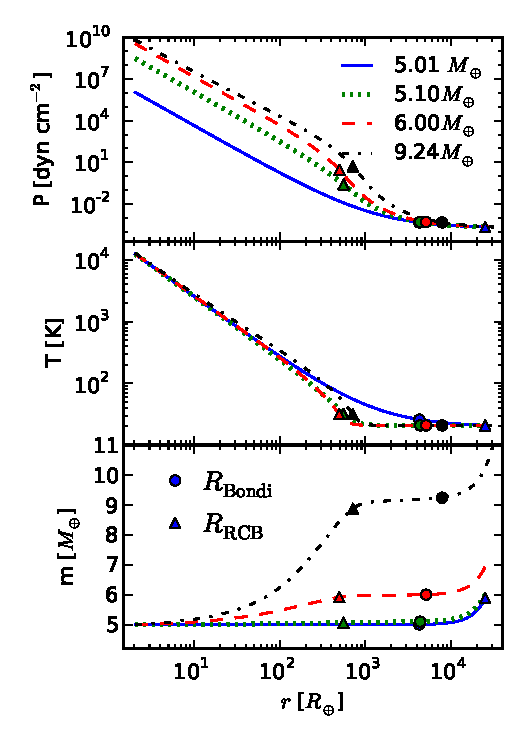
\includegraphics[width=0.5\textwidth]{../../figs/ModelAtmospheres/RadSelfGravPoly/PaperFigs/PTm_profiles_v2_smallM.pdf}
%\vspace{-0.5in}
\caption{Radial profiles of atmospheric pressure, temperature and enclosed mass (core included) for a $5 M_{\oplus}$ core at $a=60$ AU.   Solid, dotted, dashed and dot-dashed lines correspond to solutions with total mass (core and atmosphere) of $5.01 M_{\oplus}$, $5.10 M_{\oplus}$, $6.00 M_{\oplus}$ and $8.99 M_{\oplus}$, respectively.  Circles and triangles mark the locations of the Bondi radii and of the radiative-convective boundaries, respectively.  The radial profiles extend from the core to the Hill radius.} %  (See text for a description of evolution to yet higher masses.) 
\label{fig:profiles}
\end{figure}


\subsection{Atmospheric Structure}
\label{sec:profiles}
Figure \ref{fig:profiles} shows radial profiles at different stages of atmospheric growth around a $5 M_{\oplus}$ core at $60$ AU.  Quoted mass values include the core plus atmosphere within the smaller of $\RB$ or $\RH$, which for these cases is $\RB$.  The 8.99 $M_{\oplus}$ solution is the mass at which runaway growth begins according to the criteria described in \S\ref{sec:timeev}. % we can reach in our evolutionary sequence, as we explain further in \S\ref{sec:endoftime}.

The lowest mass atmosphere -- which we take as our initial state -- is fully convective with the same entropy as the disk.  In \Fig{fig:profiles} this state is the 5.01 $M_{\oplus}$ solution with no radiative zone.  Atmospheric cooling and contraction allows the accretion of more gas.  In the convective zones, higher mass solutions have lower entropy and higher pressures.  A radiative zone emerges to connect the lower entropy interior to the higher entropy disk.  \Fig{fig:profiles} shows that this radiative zone is already fairly deep in the 5.10 $M_\oplus$ solution. 
 
The atmospheric structure is well approximated by our non-self-gravitating, analytic solutions.  Deep in convective zones, \Eq{eq:deep} gives $T \propto r^{-1}$ and $P\propto r^{-1/\delad}$.  This behavior is seen in the low mass solutions in \Fig{fig:profiles}.  As explained by \Eq{eq:TPsg}, the high mass solutions show a slightly flatter profile in $T$ and also in $P \propto T^{1/\delad}$.  In agreement with \Eq{eq:cb2}, the radiative zones remain nearly isothermal, even for the higher masses.  Consequently, the pressure increases nearly exponentially with inverse depth.  


\subsection{Time Evolution}\label{sec:timeev}

\begin{figure}[tb]
\centering
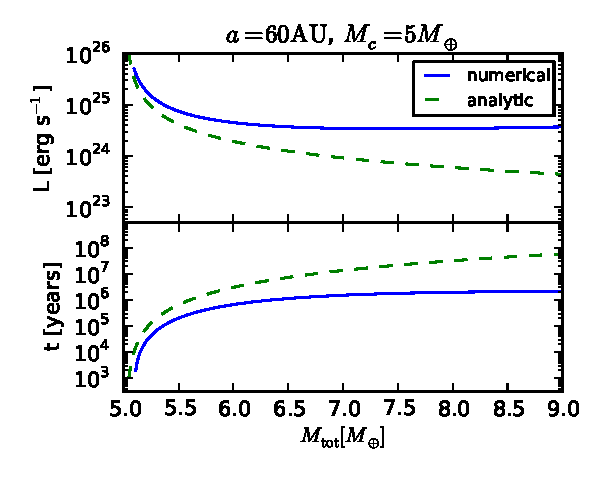
\includegraphics[width=0.5\textwidth]{../../figs/ModelAtmospheres/RadSelfGravPoly/PaperFigs/Lt_profiles_v2.pdf}
%\vspace{-0.5in}
\caption{Evolution of the luminosity and elapsed time during atmospheric growth around a $5 M_{\oplus}$ core at $60$ AU.  The luminosity is initially high, then decreases as the atmosphere grows in mass and the radiative zone becomes optically thicker.  Due to the neglect of self-gravity, the analytic model (\emph{dashed curve}) gives a further drop in luminosity and a longer evolution time.}
\label{fig:Ltplot}
\end{figure}

The cooling model of \S\ref{sec:twolayer} is used to connect solutions with different atmospheric masses into an evolutionary sequence.  \Fig{fig:Ltplot} shows the luminosity evolution and the elapsed time as a function of atmospheric mass for a $5 M_{\oplus}$ core at $60$ AU, i.e.\ the same parameters as in \Fig{fig:profiles}.  During the early stages of atmospheric growth, the luminosity drops sharply.  This behavior is seen in both the full numerical solutions (with solid lines) and the analytic model (with dashed lines).  With increasing atmospheric mass, the pressure depth of the RCB increases, along with the optical depth ($\propto \kappa P\cb)$.  Consequently, the radiative luminosity decreases.  This behavior is described in \Eqs{eq:crit}{eq:Lcb}.

At later stages of evolution, the numerical model in \Fig{fig:Ltplot} shows a flat luminosity with increasing mass and also time (not shown).  By contrast, the non-self-gravitating analytic model gives a luminosity that continues to drop as the atmosphere becomes more massive.  To understand this difference, consider the scaling of \Eq{eq:Lcb}, $L\cb \propto M\cb T\cb^4/ (\kappa\cb  P\cb)$, which holds in both cases.   Accounting for the higher enclosed mass in the self-gravitating model gives a somewhat higher luminosity, as desired.  However, the main effect is that \Eq{eq:crit} -- which describes a nearly linear relation between atmospheric mass and RCB pressure --  breaks down for self-gravitating solutions.  This behavior can be seen in the top panel of \Fig{fig:profiles} where the $P\cb$ increases significantly from 5.10 to 6.0 $M_\oplus$, but only increases relatively modestly with further growth to 9.24 $M_\oplus$.   In the higher mass solutions, the relatively low $P\cb$ values (and thus the relatively high luminosities) require an outward shift in $R\cb$, as shown in \Fig{fig:profiles}.

The accelerated growth in the numerical model, as shown in the bottom panel of \Fig{fig:Ltplot}, is also a direct result of the enhanced cooling (higher luminosities) in the self-gravitating models.  We see that self-gravity plays a very important role in atmospheric evolution, even well before the crossover mass, when $M_{\rm atm}=M\co$.
 

%Before discussing time evolution (both the elapsed time from the bottom panel of \Fig{fig:Ltplot} and the characteristic growth time of the atmosphere), we briefly discuss the effect of decreasing the atmospheric dust abundance on the atmospheric evolution.  
%AY abo e sentence is bad, we want to discuss science and not "direct traffic"

In \Fig{fig:LtvsMopacity}, the opacity normalization in \Eq{eq:opacitylaw} is reduced by factors of 10 and 100.  Lower opacities result in higher luminosities and faster evolution.  Our model thus confirms this well-established result \citep{HubBod05}.  While clearly an important effect, atmospheric dust opacities are difficult to robustly predict. Ablation of infalling solids is a dust source.  Sinks include the sequestration of solids in the core and dust settling through the radiative zone.  Grain growth both reduces dust opacities per unit mass and favors settling.  Our scenario of negligible ongoing particle accretion tends to favor low dust opacities.   To be conservative, however, our reference case considers full Solar abundances. The effect of opacity reduction on the critical core mass is described in \S\ref{sec:critical}. 

\begin{figure}[tb]
\centering
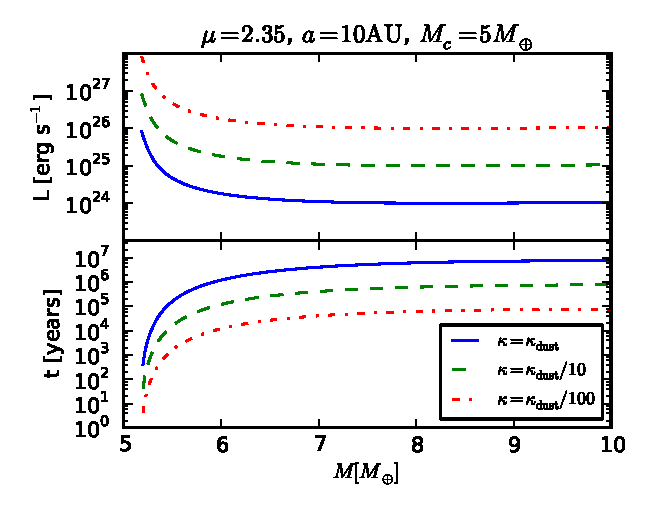
\includegraphics[width=0.5\textwidth]{../../figs/ModelAtmospheres/RadSelfGravPoly/PaperFigs/opacity_effect.pdf}
%\vspace{-0.5in}
\caption{Similar to \Fig{fig:Ltplot}, but for a $5 M_{\oplus}$ core forming at 10 AU; we show the effect of reducing the dust abundance by factors of 10 and 100 from standard Solar abundances. The reduced dust opacities give higher luminosities and faster atmospheric growth.}  %The actual magnitude of dust opacities is difficult to robustly predict.}
\label{fig:LtvsMopacity}
\end{figure}

\Fig{fig:growthtime} plots the evolution of the atmospheric growth timescale, $M_{\rm atm}/\dot{M}$,  around a $5 M_{\oplus}$ core at several locations in our reference disk model.  This instantaneous growth time shows clearly that the atmosphere spends the bulk of its time growing though intermediate atmospheric masses, $\sim 1 -3$ $M_\oplus$ in this case.  Growth times are short both early -- when the radiative zone is transparent -- and late -- when self-gravity accelerates growth.  

The fact that growth times have a well defined maximum is a characteristic of accelerating growth.  Unlike our analytic model, which must assume that runaway growth begins near the crossover mass, our numerical model allows us to measure when runaway accretion begins.  Runaway growth clearly does not begin at a universal value of $M_{\rm atm}/M\co$.  \Fig{fig:growthtime} shows that further from the star runaway growth begins at smaller $M_{\rm atm}/M\co$.  \Fig{fig:tvsM} (described in the next section) shows how the onset of runaway growth depends on core mass. 

We quantify the runaway growth timescale, $t_{\rm run}$, as the time when $M_{\rm atm}/\dot{M}$ drops to 10\% of its maximum value.  The choice of 10\% is arbitrary; the precise threshold chosen is relatively unimportant because growth continues to accelerate.


%The onset of runaway growth at high masses is also evident in \Figs{fig:Ltplot}{fig:LtvsMopacity} (bottom panels) as the flattening of the $t$ vs.\ $M_{\rm atm}$ curve.  


%peak when $M_{\rm{atm}} < M_{\rm c}$, before the crossover mass, is helpful for understanding atmospheric growth. In contrast with our analytic model, where the time to runaway accretion cannot be calculated self-consistently, the numerical model provides information about when unstable collapse occurs, i.e. when growth times decrease. It follows that the time to runaway accretion, $t_{\rm run}$, can be estimated as the time at which the atmosphere growth time $M_{\rm atm}/\dot{M}$ drops to a fraction $f$ of its maximum value. This allows for a more rigorous estimate of the runaway accretion timescale, and thus of the critical core mass, as opposed to choosing $M_{\rm atm} \sim M\co$ as the criterion for collapse. In practice, however, the continuous accelerated growth in the late stages of the atmosphere evolution renders the estimated timescale to envelope collapse, and therefore the critical core mass, insensitive to the exact choice of runaway accretion time or atmosphere mass.  Since $M_{\rm atm} < M\co$ when growth times peak, we may proceed by analogy with the analytic model and set $t=t_{\rm co}$, when $M_{\rm atm}=M\co$, as the criterion for collapse. We note that in some cases our cooling model breaks down before the crossover mass, as explained in section \S\ref{sec:endoftime}, hence evolution is stopped before $M_{\rm atm}=M\co$. However, this breakdown occurs for $M_{\rm atm} \sim 0.8-0.9 M\co$, comparable to the crossover mass, so the additional time to reach crossover is negligible. It follows that $t_{\rm run} \approx t_{\rm co}$. By analogy with the analytic results we thus choose $t_{\rm co}$ as the timescale to runaway accretion, as it will give the same numerical results as $t_{\rm run}$ and it is easier to understand in the context of other core accretion models.





\begin{figure}[tb]
\centering
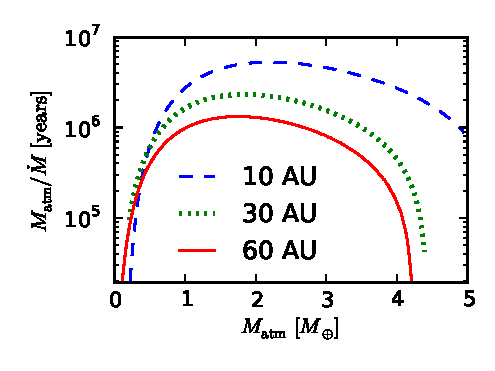
\includegraphics[width=0.5\textwidth]{../../figs/ModelAtmospheres/RadSelfGravPoly/PaperFigs/Mt_profile_temp.pdf}
%\vspace{-0.5in}
\caption{Evolution of the atmospheric growth timescale with mass around a $5 M_{\oplus}$ solid core  located at 10, 30 or 60 AU.  Growth is slowest for $M_{\mathrm{atm}} \sim 1 - 3 M_{\oplus}$, i.e.\ before the crossover mass at $M_{\rm atm} = M\co$.}
\label{fig:growthtime}
\end{figure}

\subsection{Validity of the Two-Layer Cooling Model}
\label{sec:endoftime}

We examine the  validity of our cooling model by comparing our model luminosity to the neglected luminosity, $L_{\rm negl}$,  that a more detailed model would generate in the radiative zone.  We compute $L_{\rm negl}$ from the entropy difference between successive radiative zone solutions.  We then integrate the energy equation, $\p L / \p m = - T \p S/ \p t$, over the average depth of the radiative zone.\footnote{While useful as a diagnostic, the neglected luminosity cannot reliably correct the global cooling model because the effects of $L_{\rm negl}$ on the structure of the radiative zone are still ignored.}

 \Fig{fig:coolingterms} shows that the neglected luminosity is indeed negligible during the early stages of evolution.  However, $L_{\rm negl}$ exceeds the model luminosity, $L$, at high masses, $M_{\rm atm} > 3 M_\oplus$ in this case.  Our cooling model is thus inaccurate at higher masses.  However, the model remains reasonably accurate up to the beginning stages of runaway growth, which is sufficient for our purposes of widely exploring parameter space and exploring trends.
 
The individual terms in the global cooling model of \Eq{eq:coolingglobal}, evaluated at the RCB, are also plotted in \Fig{fig:coolingterms}.  At low masses, the change in energy, $- \dot{E}$, makes the dominant contribution to luminosity.  As the mass increases, the surface terms become more significant, led by the accretion energy.  However the surface terms are everywhere smaller than $L_{\rm negl}$.  Thus wherever our model is accurate -- including the crucial early phases of growth -- surface terms are a minor correction.  The neglect of surface terms in the analytic model is thus not a serious omission.

%At even higher masses than shown in \Fig{fig:coolingterms}, our cooling model breaks down.  Mathematically, the breakdown manifests as a negative time step (due to an increase in internal entropy) when advancing to a higher atmospheric mass.  This unphysical result has no deep significance, as the neglected luminosity overwhelms the model luminosity by this point.    Effectively the model is telling us when to ignore it.  Our results are unaffected by the breakdown, which occurs comfortably after $t_{\rm run}$, our threshold for runaway growth.  

 
\begin{figure}[tb]
\centering
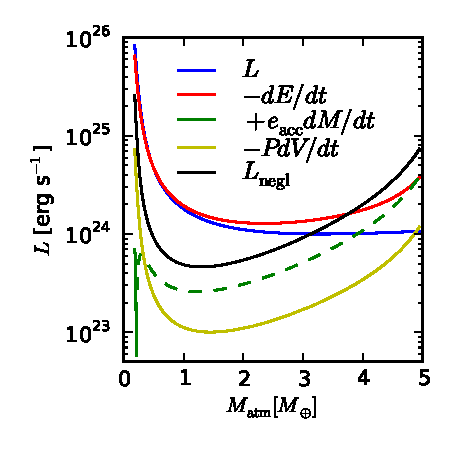
\includegraphics[width=0.5\textwidth]{../../figs/ModelAtmospheres/RadSelfGravPoly/PaperFigs/cooling_a10_Mc5_rcb.pdf}
%\vspace{-0.5in}
\caption{Individual terms in the atmospheric cooling model of \Eq{eq:coolingglobal}, for a $5 M_\oplus$ core at 10 AU.  The dashed curve for accretion energy indicates a negative contribution.  All quantities are evaluated at the RCB, except for $L_{\rm negl}$, the extra luminosity that would have been generated in the radiative zone, but is neglected in our model. The neglected luminosity is a small correction to the model luminosity $L$ for $M_{\rm atm} \lesssim 3 M_{\oplus}$.   Since these low masses dominate growth times, our model is roughly accurate.}
\label{fig:coolingterms}
\end{figure}



\section{Results for Giant Planet Formation}
\label{sec:critical}

We now use our structure and evolution models to calculate the necessary conditions for gas giant formation by core accretion.   Adopting a median disk lifetime of 3 Myr, we examine the conditions for a fixed mass core to undergo runaway gas accretion within the lifetime of the gas disk.  Our results for atmosphere growth times -- for a range of core masses and disk conditions -- are presented in \S\ref{sec:tcross}.  Section \ref{sec:critcore} gives our results for critical core masses, the minimum masses needed to accrete a massive atmosphere within the disk lifetime.

Our models focus on giant planet formation between 5 and 100 AU, as the outer disk is of particular interest for direct imaging searches.   The growth of atmospheres close to the star is also important, but spherical accretion models (including ours) are less applicable here.  In the inner disk, critical core masses increase, yet lower mass planets start to open gaps and outgrow the disk scale height, see \Eq{eq:Mth}.  These concerns prevent us from applying our model to the inner disk. 


\subsection{Runaway Growth Time Scale}
\label{sec:tcross}
The time to undergo atmospheric runaway growth, $t_{\rm run}$, sets a minimum timescale for the formation of giant planets.  Due to the accelerating nature of runaway growth, the precise threshold chosen for $t_{\rm run}$ (explained in \S ?) is of minor significance.

\begin{figure}[tb]
%\centering
\hspace{-.1in}
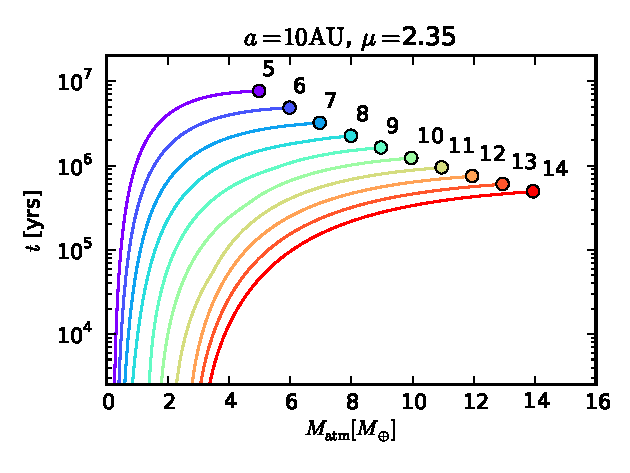
\includegraphics[width=0.5\textwidth]{../../figs/ModelAtmospheres/RadSelfGravPoly/PaperFigs/cumul_coolingtime_vs_Matm_10au_mu235.pdf}
%\vspace{-0.5in}
\caption{Time to grow an atmosphere of mass $M_{\rm{atm}}$ for cores with fixed masses between $5 M_{\oplus}$ and $14 M_{\oplus}$ (as labeled) at $10$ AU in our fiducial disk. Circles mark the runaway growth time, $t_{\rm run}$, which occurs at roughly the crossover mass, $M_{\rm{atm}} = M\co$.  Both the time to reach a fixed atmosphere mass and the runaway growth time are shorter for larger cores. For larger $M\co$, runaway growth commences at higher $M_{\rm atm}/M\co$ values.}
\label{fig:tvsM}
\end{figure}

\begin{figure}[htb]
\centering
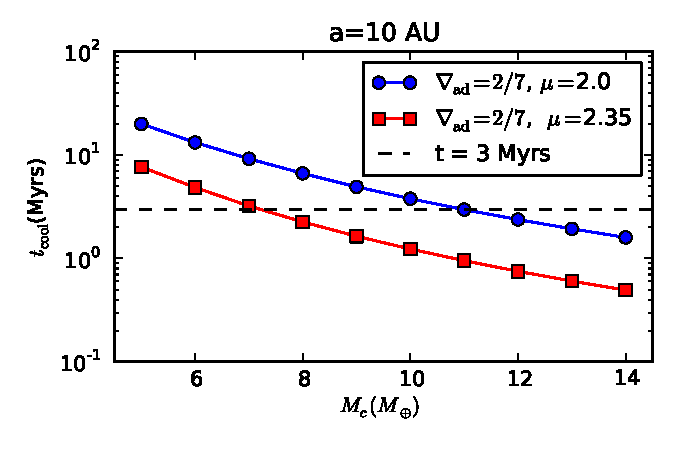
\includegraphics[width=0.48\textwidth]{../../figs/ModelAtmospheres/RadSelfGravPoly/PaperFigs/coolingtime_vs_Mc_10au.pdf}
%\vspace{-0.5in}
\caption{Runaway growth time, $t_{\rm{run}}$, vs.\ core mass at $10$ AU, for two values of the mean molecular weight.  Our numerical model (\emph{solid curves}) is compared to our non-self-gravitating analytic model (\emph{dashed curves}, from Equation \ref{eq:tcoolanf}).  A typical protoplanetary disk life time of $3$ Myr is plotted for comparison. The runaway growth time is larger for a lower mean molecular weight.}
\label{fig:tvsMcomp}
\end{figure}


\subsubsection{Effects of Core Mass}
\label{Mct}

\Fig{fig:tvsM} shows the growth of atmospheric mass with time for several core masses at $10$ AU in our fiducial disk.  Atmospheres grow faster around more massive cores due to stronger gravitational binding.  The endpoint of each curve marks $t_{\rm run}$.   Runaway growth occurs near the crossover mass, when $M_{\rm atm} \sim M\co$, in agreement with previous studies. Lower core masses undergo runaway accretion at fractionally smaller atmosphere masses. %Thus, when compared to the assumption that runaway occurs at a universal $M_{\rm atm}/M\co$ ratio,  effects that lower the critical core mass are amplified by the earlier onset of runaway growth.

\Fig{fig:tvsMcomp} shows how $t_{\rm run}$ varies with core mass, also at 10 AU.  The numerical results are plotted against our non-self-gravitating analytic model, described in \S\ref{sec:coolingan}.  The analytic model reproduces the general decline in $t_{\rm run}$ with core mass.  The numerical model, which includes self-gravity, has a somewhat steeper mass dependence.  A modest correction due to self-gravity is unsurprising, and consistent with the above-mentioned trend in $M_{\rm atm}/M\co$ ratios.  Moreover, in the analytic theory, crucial quantities like $M_{\rm atm}$ and $L$ (both roughly $\propto M\co^3$ near crossover) have non-linear dependence on core mass, offering plenty of opportunity for self-gravitational corrections.

The effect of mean molecular weight is also shown in \Fig{fig:tvsMcomp}.  A lower $\mu$ gives longer growth times, because more cooling is required to compress the atmosphere.  This effect is explained by the increase in the atmospheric scale height $\propto 1/\mu$ while the Bondi radius decreases, $\RB \propto \mu$.  For $\mu = 2.0$, which represents the idealized case of an H$_2$ atmosphere completely devoid of Helium, $t_{\rm run}$ increases by factors of $\sim 2 - 3$.  Thus fairly drastic changes in atmospheric composition are required for $\mu$ to significantly affect core accretion timescales.

%Looking ahead to our discussion of the critical core mass in \S\ref{sec:critcore}, \Fig{fig:tvsMcomp} shows that $t_{\rm run}$ equals a characteristic disk lifetime of 3 Myr for a core mass of  $M_{\rm crit} \approx 7 \, M_\oplus$  (for the standard case of $\mu = 2.35$).  


\begin{figure*}[tb]
\centering
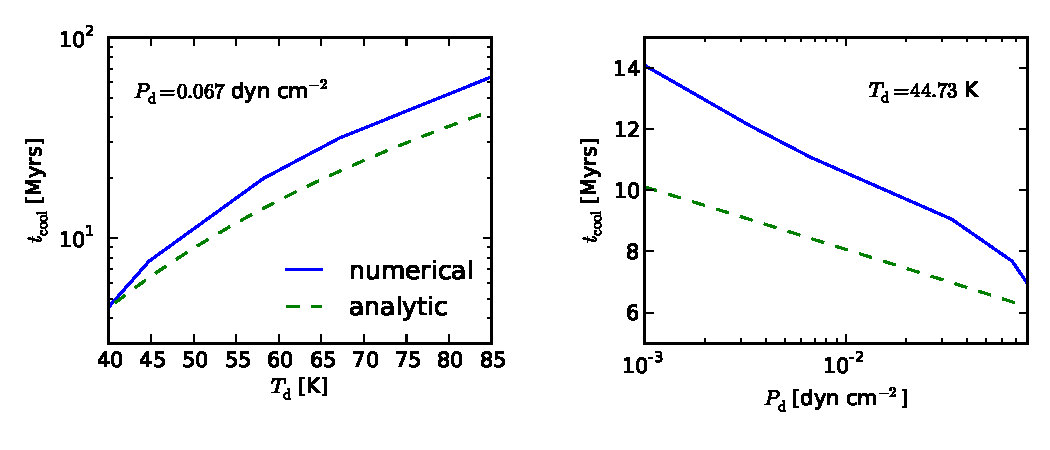
\includegraphics[width=1.\textwidth]{../../figs/ModelAtmospheres/RadSelfGravPoly/PaperFigs/TdPd_effect.pdf}
\vspace{-0.3in}
\caption{Runaway growth time as a function of disk temperature (\emph{left}) and pressure (\emph{right}) around a $M_{\rm c} = 5 M_{\oplus}$ core.   The disk pressure or temperature (\emph{left} or \emph{right}, respectively) are fixed at values for 10 AU in our disk model.   The analytic scalings given by \Eq{eq:tcoolanf} are plotted for comparison, as described in the text.  Gas accretion slows down significantly at higher temperatures, but only speeds up modestly as the disk pressure or density increase.} 
\label{fig:TPeffects}
\end{figure*}

\subsubsection{Effects of Disk Temperature and Pressure}
\label{sec:TPeffects}

\Fig{fig:TPeffects} shows how the runaway accretion time varies with disk temperature, $T\di$, or pressure, $P\di$, holding the other quantity fixed.   The analytic model roughly reproduces the temperature and pressure scalings, again with some discrepancies due mainly to the neglect of self-gravity.  Temperature variations are much more significant than pressure variations (note the difference in logarithmic and linear axes).  Since midplane disk conditions depend only on temperature and pressure in our model\footnote{See \Eq{eq:diskparam}.  When gap opening is considered in models of later growth stages, the orbital frequency and effective viscosity become relevant as well.}, the dominant effect of disk location is temperature.  

The decline in growth times at lower temperatures arises from a variety of competing effects.  Briefly, the larger Bondi radius and lower dust opacity at lower temperatures accelerate growth, overpowering the inherently lower cooling luminosity at lower temperatures.  Growth times depend only weakly on, but do fall slightly with, pressure.  The nearly exponential increase in pressure and density with depth through the radiative zone means that cooling, which is regulated at the RCB, has only a logarithmic dependence on disk pressure.   Section \ref{sec:coolingan} explains these effects in more detail.


\begin{figure}[htb]
\centering
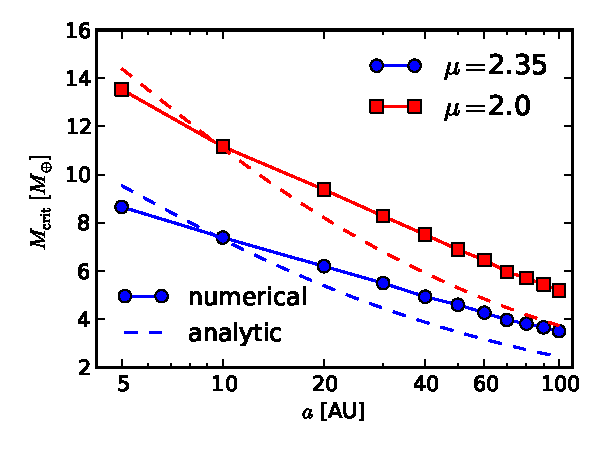
\includegraphics[width=0.5\textwidth]{../../figs/ModelAtmospheres/RadSelfGravPoly/PaperFigs/Mcrit_vs_a_3Myrs_new.pdf}
%\vspace{-0.5in}
\caption{The critical core mass as a function of semimajor axis, for a disk lifetime of $3$ Myrs and two values of the mean molecular weight ($\mu = 2.35$ is for Solar abundances). The decline in $\MC$ with distance is a robust result for standard disk models.  The analytic model, which neglects self-gravity, over-predicts the steepness of the decline.}
\label{fig:Mcvsa}
\end{figure}

\begin{figure}[htb]
\centering
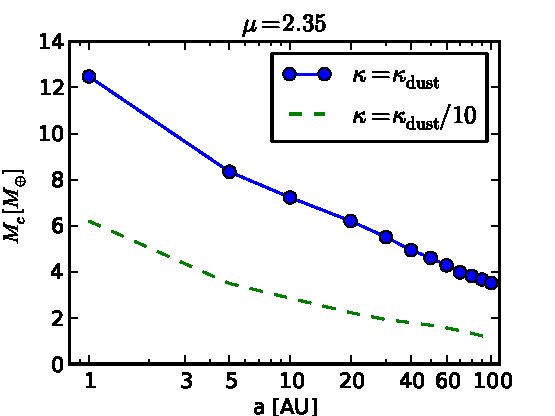
\includegraphics[width=0.5\textwidth]{../../figs/ModelAtmospheres/RadSelfGravPoly/PaperFigs/Mcrit_vs_a_3Myrs_opacity.pdf}
%\vspace{-0.5in}
\caption{Critical core masses vs. distance for standard and reduced (by a factor of ten) dust opacities.  Lower opacities give significantly lower $\MC$ values.  Atmospheric opacity remains a large uncertainty in core accretion models.}
\label{fig:Mcritopacity}
\end{figure}

\subsection{Critical Core Mass}
\label{sec:critcore}

The critical core mass declines with distance from the star, as shown in \Fig{fig:Mcvsa} for our standard disk model.   The main reason for the decline, as explained above, is that atmospheres grow faster at lower temperatures.  The lower densities and pressures in the outer disk have a much smaller effect.  Since the vast majority of disk models have a disk temperature that declines with $a$, our qualitative result is robust.   We also show that higher $\mu$ values give lower values of $\MC$.

The average power-law decline from 1 to 100 AU (not plotted) is $\MC \propto a^{-0.3}$, for both choices of $\mu$.   While not a drastic decline, the ability of distant low mass cores to accrete gas efficiently is significant for the interpretation of direct imaging surveys.  However, our model offers no guarantee of copious giant planets at large distances.  Many histories of solid accretion are possible, and solid cores may grow too slowly to allow the rapid gas accretion that we model.  

Our non-self-gravitating analytic model (dashed curves in \Fig{fig:Mcvsa}) over-predicts the steepness of the decline in $\MC$ with $a$.  This discrepancy is not surprising, as we have shown that self-gravity strongly affects evolution, even before runaway growth begins and the crossover mass is reached.

\Fig{fig:Mcritopacity} shows that reducing the opacity by an order of magnitude significantly reduces $\MC$.  Furthermore, this opacity effect is stronger at larger distances.  The opacity reduction by a factor of 10 lowers $\MC$ at 5 AU by a factor of $\sim$$2.5$ and at 100 AU by a factor of $\sim$$3.5$.  Atmospheric opacity is a dominant uncertainty in core accretion modelling.  However, unless atmospheric opacity varies significantly with disk radius, the general decline in $\MC$ with increasing $a$ should hold.  For our scenario of negligible ongoing planetesimal accretion, it is tempting to think that dust could settle out of the radiative zone, lowering the opacity \citep{podolak03}.  Nonetheless, since opacity near the RCB is a crucial factor, we speculate that convective overshoot may prevent very low opacities.

\section{Neglected Effects}\label{sec:neglected}

\subsection{Hydrodynamic Effects}\label{sec:hydro}
The neglect of hydrodynamical effects in our model is best discussed in terms of the thermal mass, $M_{\rm th}$, and the length scales introduced in \S\ref{sec:scales}.  In the low mass regime, $M\pla < M_{\rm th}/ \sqrt{3}$, where $\RB < \RH$, we assume that hydrostatic balance holds out to the outer boundary at $\RH$.   In this low mass regime, \citet[]{Orm13} calculated the flow patterns driven by stellar tides and disk headwinds.     On scales $\gtrsim \RB$ the flows no longer circulate the planet: they belong to the disk.  Nevertheless, the density structure outside $\RB$ remains spherically symmetric and hydrostatic.  Even if these flows do not destroy hydrostatic balance, they could affect the planet's cooling.  We expect such effects to be weak, as heat losses at greater depths dominate planetary cooling, but more study is needed.

At higher masses, non-hydrostatic effects become more severe.  At $M\pla \gtrsim M_{\rm th}$ planets can open significant gaps \citep{zhu13}.  At yet higher masses accretion instabilities could occur \citep{AylBat12}.  However, in this high mass regime, the spherically symmetric approximation has already broken down. %, as does our approximate cooling model (\emph{discuss elsewhere and cite}).

Thus by restricting our attention to low masses, neglected hydrodynamic effects should be minor.   Moreover since $M_{\rm th} \propto a^{6/7}$ increases with disk radius, spherical hydrostatic models like ours have a greater range of applicability in the outer regions of disks. 


\subsection{Realistic Opacities}\label{sec:op}

Treating dust (and total) opacities as a power law in temperature is a simplification.  Opacities drop by order unity when ice grains sublimate for $T \gtrsim 150$ K and they drop by orders of magnitude when silicate grains evaporate above $T \gtrsim 1500$ K \citep{semenov03, FerAle05}.  Grain growth and composition also affect opacities.  Piso et al. (in prep.) explores more realistic opacity laws.

For this work, we justify a simplified dust opacity by the cool temperatures of both the outer disk and our nearly isothermal radiative zones (see \S\ref{sec:profiles}).  While  convective interiors get significantly hotter than 1500 K, opacity does not affect the structure of adiabatic convecting regions.   A possible caveat is the existence of  radiative zones sandwiched inside the convection interior.  Such ``radiative windows" arise if the opacity drop from ice and metal grain sublimation occurs at sufficiently low pressures.  Our two-layer model ignores this possibility, but radiative windows are known to exist in hot Jupiter models \citep{burrows97, ab06} and have been seen in some core accretion models (Lissauer, personal communication).  The role of radiative windows in core accretion models remains to be explored in detail.


\subsection{Equation of State}
\label{sec:EOS}
 
Our model uses an ideal gas law and a polytropic EOS, given by \Eq{eq:idealEOS}.  However, non-ideal effects can affect atmospheric structure and evolution.  In the lower atmosphere, H$_2$ can partially dissociate at high temperatures.  In the upper atmosphere, H$_2$ rotational levels can become depopulated at lower temeratures.   Piso et al. (in prep) uses the \citet{saumon95} EOS, with extensions to lower pressures and temperatures as needed, to explore these effects.


\section{Summary} \label{sec:conclusions}

We study the formation of giant planets by the core accretion mechanism.  Our models start with a solid core that is embedded in a gas disk and no longer accreting solids.  We determine -- as a function of disk location, core mass, and the atmosphere's mean molecular weight and opacity -- whether runaway atmospheric growth can occur within a typical disk lifetime of 3 Myr.  By neglecting the accretion luminosity of planetesimals and smaller solids, we obtain the fastest allowed rate of gas accretion.  We address core accretion in the outer disk, as it is relevant to direct imaging surveys.  Our model approximations, including spherical accretion and low mass radiative exteriors with opacities dominated by dust, are tuned to conditions in the outer disk.   Our main findings are as follows:

\begin{enumerate}
\item The minimum or critical core mass, $\MC$, for giant planet formation declines with stellocentric distance in standard protoplanetary disk models.  For our reference case, the critical mass is $\sim$$8.5 M_{\oplus}$ at $a = 5$ AU, decreasing to $\sim$$3.5 M_{\oplus}$ at $a =100$ AU.  This decline roughly follows $\MC \propto a^{-0.3}$.

\item The drop in disk temperature with radial distance explains the decrease in critical core masses.  The lower pressures and densities in the outer disk only weakly suppress atmospheric growth.

\item Reducing dust opacities by a factor of 10 reduces critical core masses by a factor of $\sim$$3$.  This reduction is somewhat stronger (weaker) at larger (smaller) separations from the star.

\item A larger mean molecular weight reduces critical core masses, in agreement with \citet{HorIko11}.  If enrichment in heavy elements correlates with increased dust opacity, then the stronger opacity effect will dominate, increasing $\MC$.

\item Runaway growth begins roughly at the crossover mass, when atmosphere and core masses are equal, $M_{\rm atm} \sim M\co$, in agreement with previous work \citep{pollack96}.  Further from the star, runaway growth begins at smaller $M_{\rm atm} \sim M\co$ ratios.  For larger core masses, runaway growth begins at larger values of $M_{\rm atm} \sim M\co$.

\item Self-gravity affects atmospheric evolution before crossover.  Significant self-gravitational corrections appear when the atmosphere is only $\sim$$10 \%$ as massive as the core.

\end{enumerate}

Rapid gas accretion onto low mass cores could explain the origin of distant directly imaged giant planets \citep{marois08, lagrange10}.  However, our model does not address the details of how solid cores grow, and many possibilities exist.  For a giant planet to form with a core near the minimum mass, the core's growth must  first be rapid and then slow significantly, as in phases I and II, respectively, of \cite{pollack96}.   

Initial core growth must be fast, compared to the disk lifetime, to get a sufficiently massive core.  Subsequent slowing of core growth is required to allow the atmosphere to cool and contract.  To be more quantitative, the minimum cooling luminosity in \Fig{fig:Ltplot}, $L\approx 3.5 \times 10^{24}\;\mathrm{erg s}^{-1}$, could be cancelled by low levels of heating from solid accretion.  Specifically, a core mass doubling timescale of $\sim$$400$ Myr, or faster, would provide enough heating to stall atmospheric cooling and growth.  

Thus for giant planets to form around cores near $\MC$, core growth must stall quite severely.   The accretion and scattering of local planetesimals, combined with the inward aerodynamic drift of smaller solids past the core, offers a plausible means to sufficiently isolate the core.  On the other hand, non-negligible accretion of solids onto cores could continue for the lifetime of the gas disk.  In these cases, relatively high mass cores would remain as ice giants, akin to Uranus and Neptune.   Ongoing direct imaging surveys and their successors \citep{hinz12, macintosh12} will help discriminate among the various planet formation pathways in the outskirts of protoplanetary disks.

\acknowledgements{We thank Ruth Murray-Clay for detailed feedback and skillful proof reading. We also thank Eugene Chiang for a valuable conversation.}

\bibliographystyle{apj}
\bibliography{refs}



\appendix
\section{Derivation of the Global Energy Equation}\label{sec:globalderiv}

To derive  the global energy equation (\ref{eq:coolingglobal}) for an embedded protoplanet, we generalize the analogous calculations in stellar structure theory, e.g.\ in \S4.3 of \citet{kippenhahn90}.  For our problem, we add the effects of finite core radius, surface pressure and mass accretion.We start with the local energy equation (\ref{eq:structd}) whose more natural form in Lagrangian (mass) coordinates is $\p L/ \p m = \epsilon - T \p S /\p t$.  Integrating from the core to a higher shell with enclosed mass $M$ gives:
\begin{subeqnarray}
L - L\co &=& \int_{M\co}^M {\p L \over \p m} dm \\
&=& \int_{M\co}^M \left(\epsilon - T {\p S \over \p t} \right)dm \\
&=& \Gamma  - \int_{M\co}^M{\p u \over \p t} dm +  \int_{M\co}^M {P \over \rho^2} {\p \rho \over \p t} dm\slabel{eq:DLc}\, ,
\end{subeqnarray} 
with $\Gamma = \int \epsilon dm$ the integral of the direct heating rate and applying the first law of thermodynamics in the final step.

The global energy equation is derived by eliminating the partial time derivatives in \Eq{eq:DLc}, which are performed at a fixed mass,
in favor of total time derivatives, denoted with overdots.  %The physical distinction is that total derivatives include mass  accreted through the outer boundary.  
For instance, the surface radius $R$ of the shell with enclosed mass $M$ evolves as  
\begin{equation}\label{eq:Rdot}
 \dot{R} = {\p R \over \p t} + {\dot{M} \over 4 \pi R^2 \rho_M},
\end{equation} 
where $\p R/\p t$ gives the Lagrangian contraction of the ``original" shell, and mass accretion through the upper boundary at rate $\dot{M}$ also changes the shell location.  
%The subscript $M$  denotes quantities at the upper boundary of total mass $M$ (though it is omitted from $M$ and $R$).  
Similarly, the volume $V = (4 \pi/3)R^3$ and pressure at the outer shell evolve as
\begin{subeqnarray}\label{eq:dot}
\dot{V}_M &=&  {\p V_{\rm M} \over \p t} + {\dot{M} \over \rho_{\rm M}}  \\
 \dot{P}_M &=& {\p P_{\rm M} \over \p t} + {\p P_M \over \p m}\dot{M} =  {\p P_{\rm M} \over \p t} - {G M  \over 4 \pi R^4} \dot{M}\, .
\end{subeqnarray} 
This derivation holds the core mass and radius fixed, $\dot{M}\co = \dot{R}\co = 0$.  Therefore the core pressure satisfies
\begin{equation}\label{eq:Pcdot}
 \dot{P}\co = \p P\co / \p t \, .
\end{equation}
The internal energy integral follows simply from  Leibniz's rule as
\begin{equation}\label{eq:udot}
\int_{M\co}^{M(t)}{\p u \over \p t} dm = \dot{U}  -  \dot{M}u_M\, .
\end{equation} 
To make further progress we use the virial theorem:
\begin{equation}
\label{eq:virial}
E_G=-3 \int_{M\co}^M \frac{P}{\rho} dm + 4 \pi (R^3 P_M-R\co^3 P\co),
\end{equation}
which follows from \Eqsss{eq:structb}{eq:structa}{eq:Eg} by integrating hydrostatic balance in Lagrangian coordinates.  As an aside, the integral in equation (\ref{eq:virial}) can be evaluated for a polytropic EOS to give simple expressions for the total energy:
\begin{subeqnarray}
E&=&(1-\zeta)U+4 \pi (R^3 P_M-R\co^3 P\co) \slabel{eq:vira} \\
&=&\frac{\zeta-1}{\zeta}E_G+\frac{4 \pi}{\zeta} (R^3 P_M-R\co^3 P\co) \slabel{eq:virb}
\end{subeqnarray}
where $\zeta \equiv 3(\gamma - 1)$.  We will not make this assumption and will keep the EOS general.

To express the work integral, the final term in \Eq{eq:DLc}, in terms of changes to gravitational energy we first take the
 time derivative of \Eq{eq:virial}:
\begin{eqnarray}\label{eq:EGdot}
\dot{E}_G = 3  \int_{M\co}^M {P \over \rho^2} {\p \rho \over \p t} dm -3 \int_{M\co}^M {\p P\over \p t}{dm \over \rho} 
 -  3{P_M \over \rho_M} \dot{M}+ 3 \dot{P}_M V_M -3 \dot{P}\co V\co  + 3  P_M {\dot{ V}_M} \, . 
\end{eqnarray} 
%where the volumes, $V_M = 4 \pi R^3/3$ and $V\co = 4 \pi R\co^3/3$. 
The first integral in \Eq{eq:EGdot} is the one we want, but the next one must be eliminated.  The time derivative of \Eq{eq:Eg} (times four) gives
\begin{subeqnarray}
 4 \dot{E}_G &=&  -4 {G M \dot{M} \over R} + 4 \int_{M\co}^M {G m \over r^2}{\p r \over \p t} dm\\ 
&=&   -4 {G M \dot{M} \over R} + 4 \pi \int_{M\co}^M r^3{\p \over \p m}{\p P \over \p t} dm \slabel{eq:4EGb} \\
&=&  -4 {G M \dot{M} \over R} -3  \int_{M\co}^M {\p P\over \p t}{dm \over \rho}  + 3 V_M {\p P_M \over \p t} -3 V\co {\p P\co \over \p t} \slabel{eq:4EGc}
\end{subeqnarray} 
where \Eqs{eq:4EGb}{eq:4EGc} use hydrostatic balance  and integration by parts.

%To eliminate the time derivates of pressure, we take the time derivative of the hydrostatic balance equation for $\p^2 P / \p m\p t$ and integrate over $4\pi r^3 dm$ (as in the virial equation derivation) to get
%\begin{equation}\label{eq:dHBdt}
%3 \dot{P}_M V_M -3 \dot{P}\co V\co -3 \int_{M\co}^M {\p P\over \p t}{dm \over \rho}  = 4 \dot{E}_G + 4{G M \over R} \dot{M}  \, .
%\end{equation} 
%Combining \Eqs{eq:EGdot}{eq:dHBdt} gives 
%\begin{eqnarray}\label{eq:rhodot}
%\int_{M\co}^M {P \over \rho^2} {\p \rho \over \p t} dm  &=& - \dot{E}_G - {4 \over 3}{G M\over R} \dot{M} + {P_M \over \rho_M} \dot{M} -  P_M \dot{V}_M  \, , \nonumber \\
%&=&- \dot{E}_G - {4 \over 3}{G M\over R} \dot{M}  -  P_M {\p V_M \over \p t}  \, ,
%\end{eqnarray} 
%where the final step uses \Eq{eq:Rdot}.

Subtracting \Eqs{eq:udot}{eq:4EGc} and rearranging terms with the help of \Eqsss{eq:Rdot}{eq:dot}{eq:Pcdot} gives
\begin{eqnarray}\label{eq:PdVint}
\int_{M\co}^M {P \over \rho^2} {\p \rho \over \p t} dm  &=&  - \dot{E}_G - {G M \dot{M} \over R} - P_M {\p V_M \over \p t} \,  .
\end{eqnarray} 
Combining \Eqsss{eq:DLc}{eq:udot}{eq:PdVint}, we reproduce \Eq{eq:coolingglobal} with the accreted specific energy $e_M \equiv u_M - GM/R$.  

\section{Analytic Cooling Model Details}\label{sec:analytic}
%TODO (academic): Figure out if theta < 1 is actually required? Should be but need to check

\subsection{Isothermal Atmosphere}
\label{iso}

We consider the structure of a non self-gravitating isothermal atmosphere that extends outward from the radiative-convective boundary RCB and matches onto the disk density, $\rho_{\rm d}$, at a distance $r_{\rm fit} = n_{\rm fit} \RB$, where $R_{\rm B}$ is the Bondi radius defined in equation (\ref{eq:RB}). From equation (\ref{eq:structa}) the resulting density profile is
\begin{equation} \label{eq:rhoiso}
\rho = \rho_{\rm d} \exp \left({R_{\rm B} \over r} - {1 \over n_{\rm{fit}}} \right) \approx   \rho_{\rm{d}} \exp \left(R_{\rm B} \over r  \right),
\end{equation} 
where the approximate inequality is valid deep inside the atmosphere ($r \ll \RB$) for any $n_{\rm fit} \gtrsim 1$.  However, the choice of boundary condition does have an order unity effect on the density near the Bondi radius. 

The mass of the atmosphere is determined by integrating equation (\ref{eq:structb}) from the RCB to the Bondi radius using the density profile (\ref{eq:rhoiso}) and can be approximated as
\begin{equation} \label{eq:MatmISO}
M_{\rm iso} \approx 4 \pi \rho\di {R\cb^4 \over R_{\rm B}} e^{R_B/R\cb} = 4\pi \rho\cb \frac{R\cb^4}{R_{\rm B}}
\end{equation}
with $\rho\cb$ the density at the RCB.
This result is the leading order term in a series expansion. By comparing the expression above and \Eq{eq:Matman} under the assumption that $R\cb \ll R_{\rm B}$, we see that the mass of the outer radiative region (which is nearly isothermal) is negligible when compared with the atmosphere mass in the convective layer, as stated in Section \ref{sec:coolingan}.
% Furthermore, because the atmospheric scale-height at $R\co$ is $H_\rho = |dr /d\ln\rho| = R\co^2/R_B$, the result is intuitively the correct order of magnitude.
%Planets can attract massive atmospheres if $\theta\co \equiv R_B/R\co \gg 1$.  

\subsection{Temperature and Pressure Corrections at the Radiative-Convective Boundary}
\label{RCBcorr}

%\subsection{Temperature Contrast at Convective Boundary}
In this section we estimate the temperature and pressure corrections at the RCB due to the fact that the radiative region is not purely isothermal. From equation (\ref{eq:delrad}), we express the radiative lapse rate
\begin{equation}\label{eq:delradan}
\delrad = {3 \kappa P \over 64 \pi  G M \sigma T^4} L = \nabla\di {P/P_{\rm d} \over (T/T_{\rm d})^{4-\beta}},
\end{equation}

\noindent where the second equality follows from the opacity law (\ref{eq:opacitylaw}) and $\nabla_{\rm d}$ is the radiative temperature gradient at the disk:

\begin{equation}
\label{eq:delo}
\nabla \di \equiv \frac{3 \kappa(T{\di}) P{\di}}{64 \pi G M \sigma T_{\rm d}^4} L.
\end{equation}
Here $M$ is the total planet mass. Since our analytic model neglects self-gravity, $M=M\co$ and therefore $\nabla\di$ is constant. From equation (\ref{eq:delradan}) and $\delrad=d \ln T / d\ln P$, the temperature profile in the radiative region integrates to
\begin{equation}\label{eq:radTP}
\left(T \over T_{\rm d}\right)^{4-\beta} - 1 = {\nabla\di \over \nabla_\infty} \left( {P \over P_{\rm d}} - 1 \right) \, ,
\end{equation} 
where $\nabla_\infty = 1/(4-\beta)$ is the radiative temperature gradient for $T ,P \rightarrow \infty$.
Applying \Eqs{eq:delradan}{eq:radTP} at the RCB (where $\delrad = \delad$) under the assumption that $P\cb \gg P_{\rm d}$ results in  $T\cb=\chi T\di$ as in \Eq{eq:Tcb}, with $\chi$ defined in \Eq{eq:chi}.

The pressure at the RCB follows from \Eqs{eq:radTP}{eq:Tcb} as
\begin{equation}
\label{eq:Pcbapprox}
{P\cb\over P_{\rm d}} \simeq {\delad/\nabla\di \over 1 - \delad/\nabla_\infty}.
\end{equation} 
%This pressure contrast can be quite large since $\nabla_{\rm d} \ll 1$.
 We can eliminate $\nabla\di$ from equation (\ref{eq:Pcbapprox}) to obtain a relation between temperature and pressure in the radiative zone as a function of the RCB pressure $P\cb$. From \Eq{eq:radTP}, it follows that
 \begin{equation}\label{eq:TP}
{T \over T_{\rm d}} = \left[1 + {1 \over {\nabla_\infty \over \delad} - 1} \left({P \over P\cb} -  {P_{\rm d} \over P\cb}\right) \right]^{1 \over 4-\beta}\, .
\end{equation} 
 We can then determine the radius of the convective boundary $R\cb$ from the \Eq{eq:structa} as 
\begin{equation}\label{eq:RCBint}
{R_B \over R\cb} = \int_{P\di}^{P\cb} {T \over T_{\rm d}} {dP \over P}\, .
\end{equation}
Evaluating the integral leads to 
\begin{equation}\label{eq:Rcb}
{R_B \over r\cb} = \ln \left(P\cb \over P\di \right) - \ln \theta \, ,
\end{equation} 
with an extra correction term $\theta < 1$, when compared to an isothermal atmosphere (see Equation \ref{eq:rhoiso}). From this we arrive at the relation between $P\cb$ and $P\di$ given by Equation (\ref{eq:PcbRcb}). As opposed from the temperature correction factor $\chi$, an analytic expression for  $\theta$ cannot be obtained. Estimates for $\chi$ and $\theta$ for different values of the exponent $\beta$ in the opacity law (\ref{eq:opacitylaw}) are presented in Table 1.

%As shown in section \S\ref{iso, an isothermal atmosphere gives a simple logarithmic dependence on $P\cb$.  However, using \Eq{eq:TP} in the integral gives

% The form we chose for the correction term allows us to relate the disk and radiative-convective boundary pressures as :
% \begin{equation}\label{eq:PcbRcb}
%P\cb = \theta P_{\rm d} e^{R_B/R\cb} \, .
%\end{equation}   
%In the $P\cb \gg P_{\rm d}$ limit, the correction term is an order unity constant that depends on $\alpha$, $\beta$ and $\delad$. Similarly to the temperature correction factor $\chi$,  $\theta$ accounts for the fact that the radiative region is not perfectly isothermal. For $\delad=2/7$, $\alpha=0$ and $\beta=2$, we find $\theta \approx 0.556$. Values of $\theta$ for other choices of $\beta$ are summarized in \App{sec:analytic}.  A simple analytic expression for $\theta$ is not possible.  




\subsection{The Opacity Effect}
\label{opacityan}
A  lower opacity  decreases the critical core mass.  Reducing the opacity by a factor of one hundred results in a critical core mass one order of magnitude lower than in the standard ISM case, specifically  $\MC \approx9 M_\oplus$ for the parameters in \Eq{eq:Mcrit}.  The reduction is not  as strong as the nominal scaling would imply, $0.01^{3/5} \approx 0.06$, because $\xi$ increases.

Even with significantly lower opacities, radiative diffusion remains a good approximation at the RCB. For $\beta = 2$, we estimate the optical depth as
\begin{equation}
\tau\cb \sim {\kappa\cb P\cb \over g} \sim 7 \times 10^4 {F_T^4 F_\kappa \over \left(\mc \over 10 \right) \left(\au \over 10\right)^{12 \over 7}}, 
\end{equation} 
where $P\cb \sim P_M$ for a self-gravitating atmosphere and $g \sim G M\co/R_B^2$, with both approximations good to within the order unity factor $\xi$.  We see that $\tau\cb \gg 1$ even for $F_\kappa \lesssim 0.01$ out to very wide separations, hence the atmosphere remains optically thick at the RCB.

%A hotter disk would increase core masses.  Instead of our passive disk model, adopting the standard Hayashi temperature profile would increase core masses by $\sim 50\%$.  A hotter accretion phase would further increase core masses, but such phases are presumably short lived.

\subsection{Surface Terms}
\label{surfterms}
In this section we check the relevance of the neglected surface terms in \Eq{eq:coolingglobal}.  We first show that accretion energy is only a small correction at the RCB, which is where we apply our cooling model. A rough comparison (ignoring terms of order $\xi$) of  accretion luminosity vs. $\dot{E}$ gives
\begin{equation}
{G M \dot{M} \over R \dot{E}} = {G M  \over R}{dM \over dE} \sim {G M\co^2 \over R_B E}{P\cb \over P_M} \sim \sqrt{R\co \over R_B} \ll 1,
\end{equation} 
where we assume $P\cb \sim P_M$  for a massive atmosphere.  Accretion energy at the protoplanetary surface is thus very weak for marginally self-gravitating atmospheres, and even weaker for lower mass atmospheres.  A similar scaling analysis shows that the work term $P_M \p V_M/\p t$ is similarly weak.  Nevertheless, our numerical calculations include these surface terms in a more realistic and complete model of self-gravitating atmospheres.


%\subsection{Hydrogen Dissociation}
%The dissociation of molecular hydrogen deep in the atmospheres of accreting protoplanets plays a significant role in the energetics of core accretion.  In the high density regions $r  \ll R\cb$ of a convective atmosphere, the thermal plus gravitational energy scales as
%\begin{equation}
%dE = -4 \pi \nabla_{\rm ad}^{1/\nabla_{\rm ad}} \rho\cb R_B'^{1/(\gamma-1)} r^{\frac{2\gamma - 3}{\gamma - 1}} {dr \over r}
%\end{equation} 
%If $\gamma < 3/2$ then the main contribution to the energy is at the bottom of the atmosphere, i.e.\ the core.  This is the case for a diatomic ideal gas ($\gamma = 1.4$) or a solar mixture of hydrogen and helium ($\gamma \approx 1.43$).  However a monatomic gas has $\gamma = 5/3 > 3/2$.  In this case, the atmosphere's energy is no longer concentrated near the bottom, but will be concentrated near the top of the convective zone.
%
%A likely structure is an atmosphere that is dissociated near the base, but becomes molecular near the top of the convective zone.  In this case the atmosphere's energy budget would be concentrated near the atomic to molecular transition.
%
%The energy required to dissociate a hydrogen molecule, $I = 4.467$ eV can be significant to the overall energy budget.
%Since
%\begin{equation}
%{I \over \nabla_{\rm ad} G M\co (2 m_{\rm H})/r} \approx 3 \left(M\co \over 10 M_\oplus \right)^{-2/3} {r \over R_{\rm c}}
%\end{equation} 
%we see that this energy is always relevant.
%
%We can use the Saha equation to determine where dissociation is significant,
%\begin{equation}
%{n_{\rm H}^2 \over n_{\rm H_2}} = \left(\pi m_{\rm H} k T \over h \right)^{3/2} e^{-I/(kT)}
%\end{equation} 
%We introduce a reaction coordinate $\delta$ so that $n_{\rm H} = 2 \delta n_o$ and $n_{\rm H_2} = (1-\delta) n_o$ with $n_o = \rho X/(2 m_{\rm H})$ the number density when all hydrogen is molecular.  We express equilibrium as
%\begin{equation}
%{\delta^2 \over 1-\delta} = f_\mu {P_{\rm diss}(T) \over P}
%\end{equation} 
%with the characteristic pressure below which dissociation occurs is
%\begin{equation}
%P_{\rm diss} = {\left(kT\right)^{5/2} \over 4} \left( \pi m_{\rm H} \over h^2\right)^{3/2}  e^{-I/(kT)}
%\end{equation} 
%and the order unity factor
%\begin{equation}
%f_\mu = 2\delta + (1-\delta) + Y/2 + Z/\mu_Z
%\end{equation} 
%accounts for variations in the mean molecular weight with dissociation.  (Take $\mu_Z = 31/2$, but not too significant.)
%
%Thus dissociation occurs where $P \lesssim P_{\rm diss}(T)$.  At disk temperatures (say 150 K) the dissociation pressure is negligibly small ($\sim 10^{-141}$ dyne cm$^{-2}$) and no dissociation occurs.  However at core temperatures the dissociation pressure is quite large especially for massive cores.  Dissociation is guaranteed.


\begin{deluxetable}{cccccc}  % <--- column justification (center/left/right)
\gdef \numcols {6}
\tablecolumns{\numcols}
\tablecaption{Parameters Describing Structure of Radiative Zone.}
\tablehead{   \multicolumn{\numcols}{c} {$\gamma = 7/5$ ($\delad = 2/7$)} }  
\startdata
 $\beta$   		 &1/2  	& 3/4 &1   		& 3/2  		& 2   \\
 $\nabla_\infty$ & 2/7 \tablenotemark{a}  	&  4/13	& 1/3 	& 2/5 	 	& 1/2 \\
 $\chi$ 		 & \nodata &  2.25245 &1.91293 	& 1.65054 	& 1.52753 \\
 $\theta $  		 &\nodata   & 0.145032	&0.285824   &0.456333   & 0.556069   \\
\enddata
\tablenotetext{a}{Since $\delad = \nabla_\infty$ there is no convective transition at depth for this case.}
\end{deluxetable}



%\subsection{Estimate of Atmosphere Mass Outside the Bondi Radius}
%
%Here we consider the mass exterior to the Bondi radius.  For a meaningful evaluation we only include the mass coming from the overdensity relative to the background density.  The resulting external mass for an isothermal atmosphere is
%\begin{subeqnarray}
%M_{\rm ext} &=& 4 \pi \int_{\RB}^{r_{\rm fit}} (\rho - \rho\di) r^2 dr \\
%&=& M\co \theta\co \int_1^{n_{\rm fit}} 3 \left[ \exp \left({1 \over x} - {1 \over n_{\rm fit}}\right) - 1 \right] x^2 dx  \nonumber \\
%&\equiv& M\co \theta\co I(n_{\rm fit})
%\end{subeqnarray} 
%where $\theta_c=R_B/R_{\rm c}$ and the dimensionless integral $I(n_{\rm fit})$ obeys the limits $I(1) = 0$ and $I \rightarrow n_{\rm fit}^2/2$ as $n_{\rm fit} \rightarrow \infty$.  Since this external mass does not converge, the choice of an outer boundary does matter in principle.  In practice, however, the assumption that   $r_{\rm fit} = R_{\rm H}$ limits $n_{\rm fit}$ to modest values
%\begin{equation}
%n_{\rm fit} = {R_{\rm H} \over \RB} \approx 1.3 {\aun{10}^{4/7} \over \mcn{10}^{2/3}}{F_T \over  m_\ast^{1/3}}.
%\end{equation} 
%Since for instance $I(2) = 1.1$, these modest $n_{\rm fit}$ values will only produce a small external mass.

\end{document}



